\documentclass[withoutpreface,bwprint]{cumcmthesis}
\usepackage{amsmath,amssymb}
\usepackage{graphicx}
\graphicspath{{../figures/}}
\usepackage{booktabs}
\usepackage{multirow}
\usepackage{longtable}
\usepackage{tabularx}
\usepackage{float}
\usepackage{subcaption}
\usepackage{url}
\usepackage{listings}
\hypersetup{hidelinks}
\title{面向算电协同的多目标调度优化研究}
\author{题号：C}
\date{}
\begin{document}
\maketitle
\begin{abstract}
针对六区域异构 AI 任务与新能源、储能、电网的耦合调度，本文构建“rolling-origin 闭环预测—语义唯一公共候选多遍搜索—来源显式储能动态规划—按情景交替搜索”的可复算框架。问题一在最终测试前以 8 个 expanding-window 原点完成 1584 次闭环评价；Macro-WAPE、Micro-WAPE 和 System Aggregate WAPE 分别为 0.8069、0.6312 和 0.2794，独立基础调度覆盖 50000 个任务。问题二构造 120000 行且语义零重复的公共候选池，五方向按相同顺序完成 6 个 pass，并以共同第 5 遍正式比较。问题三统一拆分新能源充电、网充、新能源售电和储能售电，以净电网交换定义峰值与波动，采用相邻 SOC 对动态规划真正优化净波动，并以可用 SOC 区间计算 EFC；修正后加权理想点选择平衡策略，成本、新能源率、净波动和 EFC 分别为 $-4.541740\times10^8$ 元、0.693131、22150.241 MW 和 92.401。问题四对 17 个情景统一复算能源与服务指标，并按由松到严继承碳候选；20\%、30\% 档仅标记声明搜索内未找到达标候选。两次无墙钟运行的 106 个结构化产物无语义差异，results.json 哈希均为 \texttt{c63996f2...389e}。结果只表示声明有限候选内的 scenario-feasible 解，不构成全局最优或完整 Pareto 前沿。
\end{abstract}
\keywords{异构 AI 任务；rolling-origin；闭环预测；算电协同；多目标调度}
\clearpage
\section{问题重述}

随着人工智能推理与训练任务持续增长，数据中心的算力分配已经与能源供给、碳排放和通信服务质量形成紧密耦合。题目给出了六个区域的 GPU 容量、IT 与设施功率边界、逐时非 AI 负荷、PUE、电价、碳强度、新能源出力、购售电限制、储能参数以及区域间单向网络时延，同时提供了三类异构 AI 任务的到达时刻、GPU 需求、预计持续时间、来源区域、最大允许时延和完成期限。需要在满足物理边界与服务约束的条件下，合理确定任务的执行区域和开工时刻，并协调新能源、储能及电网购售电行为。

整个运行过程具有明确的分层时间边界。第 $0$ 至第 $2399$ 小时构成任务到达主时域，第 $2400$ 至第 $2405$ 小时不再接收新任务，仅允许此前到达的弹性任务继续执行并完成结清；第 $2406$ 小时不得安排任何任务，只用于电力运行和储能终端状态结算。所有任务均不可拆分、不可抢占，也不得在执行过程中迁移。实时推理任务必须在到达时刻立即开工，批量推理与 AI 训练任务可以在允许范围内延迟，但其完成时点不得超过任务截止时间和系统统一终点。

对于问题一，需要按区域和任务类型统计 GPU 需求的规模、分布及时间规律，建立短期需求预测模型，并按照时间顺序完成模型训练、验证与最终测试。预测结果仅用于模型精度评价，最后 $24$ 小时的基础调度必须使用第 $2376$ 至第 $2399$ 小时的实际到达任务。调度时还需根据分钟级持续时间计算任务与各小时的真实重叠，据此分别审计瞬时 GPU 占用和小时电量，并展示任务实际起止时刻、执行区域及区域 GPU 利用情况。

对于问题二，需要使用全体实际任务和逐时电力参数重新构造碳感知调度方案。在任务唯一执行、实时任务即时开工、网络时延、GPU 容量、IT 功率、设施功率及完成时限均得到满足的基础上，系统运行成本、购电碳排放、有效网络时延和新能源利用率应被统一复算。问题二不配置储能，新能源被用于直接供能、区域外送或弃置，不足负荷由电网购电补足，且购电与售电行为必须服从区域边界及互斥要求。

对于问题三，任务调度不再作为本问决策变量；程序读取问题二五个 direct 正式方案的哈希，并按方法合同选择 formal balanced 的逐时设施负荷作为共同储能输入。需要在储能初始状态、荷电状态递推、容量和功率边界、充放电互斥、购售电互斥以及终端能量不透支等条件下，确定逐区域逐时的充电、放电、购电、售电、新能源分配和弃电策略，并将含储能方案与无储能比较状态在成本、碳排放、峰值净购电功率和负荷爬坡方面进行比较。

对于问题四，需要把任务迁移与开工、设施负荷、新能源分配、储能运行以及购售电决策纳入同一框架，在运行成本、碳排放、网络时延、服务质量、新能源利用率和区域峰值净购电之间进行权衡。碳约束、电价机制与新能源波动等情景应从同一联合基准独立重构，并在相同任务集、容量边界、功率映射和评价口径下接受完整审计，从而辨析不同外部条件对任务迁移方向、执行窗口与能源行为的影响。
\section{问题分析}

\subsection{数据预处理}
普通空白值在未经核验前视为不可裁决缺失，不自动替换为零。仅当互斥进流与出流字段满足“本行孤立事件、另一列明确非零，且备注、相邻记录和全表口径共同支持互斥解释”时，才将空白认定为结构零；所有处理均保留字段来源与审计记录。
本题同时包含任务级离散决策、分钟级连续占用和小时级能源结算。若把任务直接压缩为小时平均负荷，会漏掉只在小时内短暂重叠却造成瞬时 GPU 峰值的任务；若把所有触及某小时的任务都按整小时计费，又会高估 AI 电量。因此本文先保留任务的真实起止区间，再用“是否正重叠”审计瞬时容量，用“实际重叠时长”核算 GPU-hour 和电量，最后把重建负荷传给能源模型。

\subsection{问题一：预测与末端调度分离}
预测对象是区域—任务类型—小时的到达 GPU 需求。训练、验证、测试必须按时间顺序切分，且多步预测时后续滞后项只能使用此前预测值，不能回填测试真值。日周期与周周期朴素模型提供可解释基线，Huber 回归处理尖峰需求并通过验证集选择超参数\cite{huber1964robust}。预测只用于精度评价；最后 24 小时调度仍读取第 2376 至 2399 小时实际到达的 538 个任务，从而避免“以预测量替代真实任务”的口径错误。

末端任务可能跨越第 2399 小时，因此调度时域延伸到第 2405 小时；第 2406 小时只用于能源和 SOC 结算。实时推理必须到达即开工，弹性任务可在到达与截止之间选择整数开工时刻。候选区域还需同时通过单向时延、GPU、IT 功率和设施功率下界筛选。

\subsection{问题二：同一 CandidateID 流上的公平比较}
问题二的首要风险是把“任务触及某小时的瞬时功率”误作该小时整小时电量。本文分别维护瞬时 GPU、瞬时 IT 功率、按重叠时长累计的 AI 电量和由电量换算的设施小时平均功率。五个直接方向从同一 Q1 基线出发，并按目标无关的 round-robin 分层顺序读取完全相同的 CandidateID 前缀；前 50000 行先覆盖全部任务，随后两层再扩展同一任务的时间与区域候选。直接碳方向与额外多起点强化分开，后者不进入公平横向表。

\subsection{问题三：正式平衡负荷上的储能比较}
问题三读取五个 Q2 direct 方案的正式哈希，并按预先声明的下游合同把 formal balanced 的设施负荷作为共同输入。储能候选仍包含 no-action、成本、碳、新能源、峰值、爬坡和平衡七种策略；轨迹先去重和候选内支配筛选，再以统一加权理想点距离选择，避免按方案名称指定答案。

\subsection{问题四：按情景动态重建邻域}
联合问题中，任务方案改变设施负荷，储能轨迹又改变任务移动的边际电价和边际碳信号。固定若干预制任务方案再逐情景挑选，会切断这种反馈。本文对每个情景从唯一共同任务基线和真实初始 SOC 独立重启；不存在预制的两个替代任务方案。对当前负荷分别计算成本、平衡、新能源三类储能政策，按 Q4 自身的加权理想点规则选择，再依据所选轨迹形成价格、碳、购电和弃电信号，动态生成 600 个任务候选。接受改进后重建下一轮邻域。最多 8 轮，连续 2 轮无改善即停止。

17 个情景覆盖基准、4 个碳约束水平、3 个峰谷价差、3 个售电机制、3 个新能源水平，以及种子 2026、2027、2028 的新能源波动。正常联合基准若为正碳，四档碳目标直接以该基准定义；若为零碳，才改用新能源缩放 0.8 的短缺压力基准，且不与正常基准混淆。每类情景输出唯一任务调度数、唯一储能轨迹数、机制活跃性和退化原因。碳目标未达到只能表述为“声明启发式内未达到”，不能据此推断数学不可行。

\subsection{四问衔接与证据边界}
四问共享任务重叠、设施负荷、能源守恒和审计函数，但不直接拼接决策结果。问题二以问题一可行基线启动；问题三与问题四均读取修复后的五个 direct 正式哈希，并以问题二 formal balanced 的设施负荷为共同基线，统一使用 21 状态网格，但在每个情景和每轮独立重选三类储能政策。输出可信性来自结构化结果、逐行 CSV、完整约束审计和两次隔离复算。由于不存在独立 Oracle，最高可信等级限定为 scenario-feasible。
\section{模型假设}

\begin{enumerate}
\item 题目附件中给出的任务需求、设备容量、功率参数、电价、碳强度和新能源出力等数据，在其给定精度内视为可靠的确定性参数；除情景分析中主动设置的扰动外，不考虑设备故障、通信中断等突发事件。
\item 调度以小时为决策步长，任务在整数小时选择开工时刻；任务一旦开始便连续执行，不允许拆分、抢占、暂停或中途迁移，跨小时能耗按照任务与各小时的实际重叠时长计算。
\item 同类任务的单位 GPU 功率、各区域 PUE 和区域间单向网络时延在研究期内保持不变；不考虑网络拥塞、带宽限制以及数据传输产生的额外能耗和费用。
\item 购售电价格、电网碳强度、可用新能源和固定负荷在单个小时内保持恒定，各区域独立满足能源平衡；不考虑跨区域电力潮流、线路损耗及设备全生命周期碳排放。
\item 储能充放电效率采用附件给定值并在研究期内保持不变，忽略储能自放电和容量衰减；为避免通过透支期末电量获得虚假收益，规定调度结束时储能 SOC 恢复至初始水平。
\end{enumerate}
\section{符号说明}

\begin{table}[H]\centering
\fontsize{8}{9}\selectfont
\renewcommand{\arraystretch}{0.88}
\caption{核心符号说明}\label{tab:symbols}
\begin{tabular}{p{0.27\textwidth}p{0.62\textwidth}}
\toprule
符号 & 含义\\
\midrule
$i,r,t,s$ & 任务、区域、小时及候选开工时刻索引\\
$x_{irs}$ & 任务 $i$ 是否在区域 $r$、时刻 $s$ 开工\\
$\omega_{it}(s)$ & 任务 $i$ 与小时 $t$ 的实际重叠时长\\
$\chi_{it}(s)$ & 任务 $i$ 在小时 $t$ 是否占用瞬时资源\\
$D_{rkt},\widehat D_{rkt}$ & 实际与预测的逐时 GPU 需求\\
$G_r^{\max}$ & 区域可用 GPU 容量\\
$P_r^{IT,\max},P_r^{F,\max}$ & 区域 IT 与设施功率上限\\
$p_k^{GPU}$ & 任务类型 $k$ 的单位 GPU 功率\\
$\pi_r$ & 区域 PUE\\
$L_{rt}^{F}$ & 区域设施负荷\\
$R_{rt}^{av}$ & 可用新能源功率\\
$G_{rt}^{buy},G_{rt}^{sell}$ & 电网购电与售电功率\\
$C_{rt},D_{rt}$ & 储能充电与放电功率\\
$S_{rt},S_r^0$ & 储能 SOC 与初始 SOC\\
$\eta_r^c,\eta_r^d$ & 储能充、放电效率\\
$N_{rt}$ & 区域净购电功率\\
$C_{op},E_{CO_2}$ & 系统运行成本与碳排放\\
$U_{RE}$ & 新能源利用率\\
$J_s,Q_{service}$ & 服务目标与服务质量指标\\
$P^{peak},V$ & 峰值净购电功率与功率波动量\\
\bottomrule
\end{tabular}
\end{table}
% MMW-METHOD-CONTRACT: a25778b6e6b6690f819a190e628d6476bfd2f57c6161872472aa017c84c32a02
% MMW-ID: OBJ-Q1
% MMW-ID: OBJ-Q2
% MMW-ID: OBJ-Q3
% MMW-ID: OBJ-Q4
% MMW-ID: CON-Q1-1
% MMW-ID: CON-Q1-2
% MMW-ID: CON-Q1-3
% MMW-ID: CON-Q1-4
% MMW-ID: CON-Q1-5
% MMW-ID: CON-Q1-6
% MMW-ID: CON-Q1-7
% MMW-ID: CON-Q2-1
% MMW-ID: CON-Q2-2
% MMW-ID: CON-Q2-3
% MMW-ID: CON-Q2-4
% MMW-ID: CON-Q2-5
% MMW-ID: CON-Q2-6
% MMW-ID: CON-Q3-1
% MMW-ID: CON-Q3-2
% MMW-ID: CON-Q3-3
% MMW-ID: CON-Q3-4
% MMW-ID: CON-Q3-5
% MMW-ID: CON-Q3-6
% MMW-ID: CON-Q3-7
% MMW-ID: CON-Q4-1
% MMW-ID: CON-Q4-2
% MMW-ID: CON-Q4-3
% MMW-ID: CON-Q4-4
% MMW-ID: CON-Q4-5
% MMW-ID: CON-Q4-6
% MMW-ALGORITHM: 8原点rolling-origin闭环预测；Q1独立基础调度；五维分层任务搜索；统一理想点折中；21状态SOC动态规划；按情景动态交替有限搜索
\section{模型的建立与求解}

\subsection{统一时间口径与任务调度约束}
\subsubsection{统一时间口径}
第 $0$--$2399$ 小时为任务到达主时域，第 $2400$--$2405$ 小时只结清此前到达的弹性任务，第 $2406$ 小时不产生任务资源占用，仅用于电力运行和储能终端结算。

\subsubsection{任务调度约束}
任务 $i$ 的 GPU 数、到达时刻、持续小时数和有效截止分别记为 $g_i,a_i,h_i,F_i$，其中 $h_i=d_i/60$，$F_i=\min\{l_i,2406\}$。任务在整数时刻 $s_i$ 开工，与小时区间 $[t,t+1)$ 的重叠量为
\begin{equation}
\omega_{it}=\max\{0,\min(t+1,s_i+h_i)-\max(t,s_i)\},\qquad
\chi_{it}=\mathbf 1\{\omega_{it}>0\}.
\end{equation}
$\chi_{it}$ 用于瞬时 GPU 与功率边界，$\omega_{it}$ 用于电量。合法候选集合满足
\begin{equation}
\Omega_i=\{(r,s):s\ge a_i,\ s+h_i\le F_i,\ \ell_{o_i r}\le \ell_i^{\max},\ \omega_{i,2406}=0\}.
\end{equation}
每个任务恰选一个候选；实时推理任务必须满足 $s_i=a_i$，批量推理与 AI 训练任务可延迟开工，但必须在 $F_i$ 前完成。区域 $r$ 在小时 $t$ 的 GPU、IT 与设施功率约束为
\begin{align}
\sum_i g_i\chi_{it}\mathbf 1(r_i=r)&\le \bar G_r,\\
L_{rt}^{N}+\sum_i g_i p_{k_i}^{GPU}\chi_{it}\mathbf 1(r_i=r)&\le \bar P_r^{IT},\\
\pi_r\!\left(L_{rt}^{N}+\sum_i g_i p_{k_i}^{GPU}\chi_{it}\mathbf 1(r_i=r)\right)&\le \bar P_r^{F}.
\end{align}
AI 平均负荷则以 $\omega_{it}$ 累计。运行成本、购电碳排放与新能源利用率统一为
\begin{align}
C&=\sum_{r,t}(c^{buy}_{rt}G^{buy}_{rt}-c^{sell}_{rt}G^{sell}_{rt}),\\
E&=\sum_{r,t}\kappa_{rt}G^{buy}_{rt},\\
U&=\frac{\sum_{r,t}(R^{use}_{rt}+R^{ch}_{rt}+R^{sell}_{rt})}{\sum_{r,t}R^{av}_{rt}},
\end{align}
其中 $U$ 仅在分母为正时计算。网络时延与等待按任务 GPU-hour 加权；服务优化目标及其无量纲质量变换在问题二统一定义，实时 SLA 与按期率只作辅助说明。

\subsection{问题一预测与调度流程}
预测模型与正式调度严格分离：预测值只用于精度评价和时间稳定性检验，正式基础调度始终读取实际任务与实际逐时参数。

\subsubsection{预测候选与无泄漏选模}
对区域 $r$、任务类型 $k$ 的到达 GPU 序列 $D_{rkt}$，Huber 候选使用滞后 $1,2,3,24,48,168$ 及日、周正余弦特征：
\begin{equation}
\begin{aligned}
x_{rk,t}=\big[&D_{rk,t-1},D_{rk,t-2},D_{rk,t-3},\\
&D_{rk,t-24},D_{rk,t-48},D_{rk,t-168},\\
&\sin(2\pi t/24),\cos(2\pi t/24),\\
&\sin(2\pi t/168),\cos(2\pi t/168)\big]^{\mathsf T}.
\end{aligned}
\end{equation}
候选包括 24 小时季节朴素、168 小时季节朴素，以及 9 个 Huber 组合；Huber 参数网格为
\[
\epsilon\in\{1.10,1.35,1.75\},\qquad \alpha\in\{10^{-4},10^{-3},10^{-2}\}.
\]
题面建议的官方切分保持不变：第 0--2351 小时训练，第 2352--2375 小时验证，第 2376--2399 小时最终测试。为检查时间鲁棒性，另取预测原点
\[
2184,2208,2232,2256,2280,2304,2328,2352,
\]
在每个原点只使用此前数据拟合，并闭环递归预测后续 24 小时；进入窗口后的短滞后只读取此前预测值。每条序列按 8 个窗口的平均 RMSE、平均 MAE、平均 WAPE 和固定候选顺序确定性选模，再用第 0--2375 小时重拟合，最终测试仅使用一次且不参与排序。

18 条序列均选择 Huber，但没有一条序列在 8 个窗口中始终排名第一；选定候选的窗口第一名次数为 1--5 次，说明候选排名随预测原点变化，单窗口结论并不稳定。该结果不否定题面建议切分，而是表明额外 rolling-origin 检查具有必要性。最终测试的按任务类型误差见表~\ref{tab:q1type}。
\begin{table}[H]\centering
\caption{rolling-origin 选模后的最终测试误差}\label{tab:q1type}
\begin{tabular}{lrrr}\toprule
任务类型 & 平均 MAE/GPU & 平均 RMSE/GPU & Macro-WAPE\\\midrule
实时推理 & 2.8149 & 3.9365 & 0.7995\\
批量推理 & 12.6782 & 16.7702 & 0.7305\\
AI 训练 & 60.9916 & 81.8017 & 0.8906\\\bottomrule
\end{tabular}
\end{table}

三种 WAPE 口径并列列于表~\ref{tab:q1wape}。Macro-WAPE 先对 18 条序列分别计算再平均，因而对低基数序列敏感；Micro-WAPE 汇总 432 个观测的绝对误差与真实需求，按需求规模加权；System Aggregate WAPE 先按小时聚合 18 条序列，能刻画系统总量，但高估与低估会相互抵消，不能单独称为“总体准确率”。全部 432 个观测的总体 MAE 与 RMSE 分别为 25.4949 GPU 和 53.8961 GPU。
\begin{table}[H]\centering
\caption{最终测试的三种 WAPE 口径}\label{tab:q1wape}
\begin{tabular}{lrp{7.2cm}}\toprule
口径 & 数值 & 含义\\\midrule
Macro-WAPE & 0.8069 & 18 条序列 WAPE 的算术平均，对低基数敏感\\
Micro-WAPE & 0.6312 & 全部观测按真实需求规模加权\\
System Aggregate WAPE & 0.2794 & 逐小时系统聚合，存在误差抵消\\\bottomrule
\end{tabular}
\end{table}

图~\ref{fig:q1forecast}a 显示系统实际需求在 24 小时内存在明显尖峰，而预测曲线更平滑，说明模型能把握需求水平但会压缩峰值；这与 Macro-WAPE 高于系统聚合 WAPE 的误差抵消现象一致。图~\ref{fig:q1forecast}b 由 38016 条候选逐小时预测中筛出各序列按 8 窗口综合规则选定的 3456 条预测复算，8 个窗口的 Macro-WAPE、Micro-WAPE 和系统聚合 WAPE 分别落在 0.7642--0.9515、0.6772--0.7667 和 0.2305--0.3369。Macro 始终高于 Micro，表明低基数序列仍是主要误差来源；系统聚合口径进一步降低，说明序列间高估与低估存在抵消。三条曲线均不使用逐窗胜者，且全部窗口位于最终测试之前，因此没有利用最终测试或窗口真值选模。
\begin{figure}[H]\centering
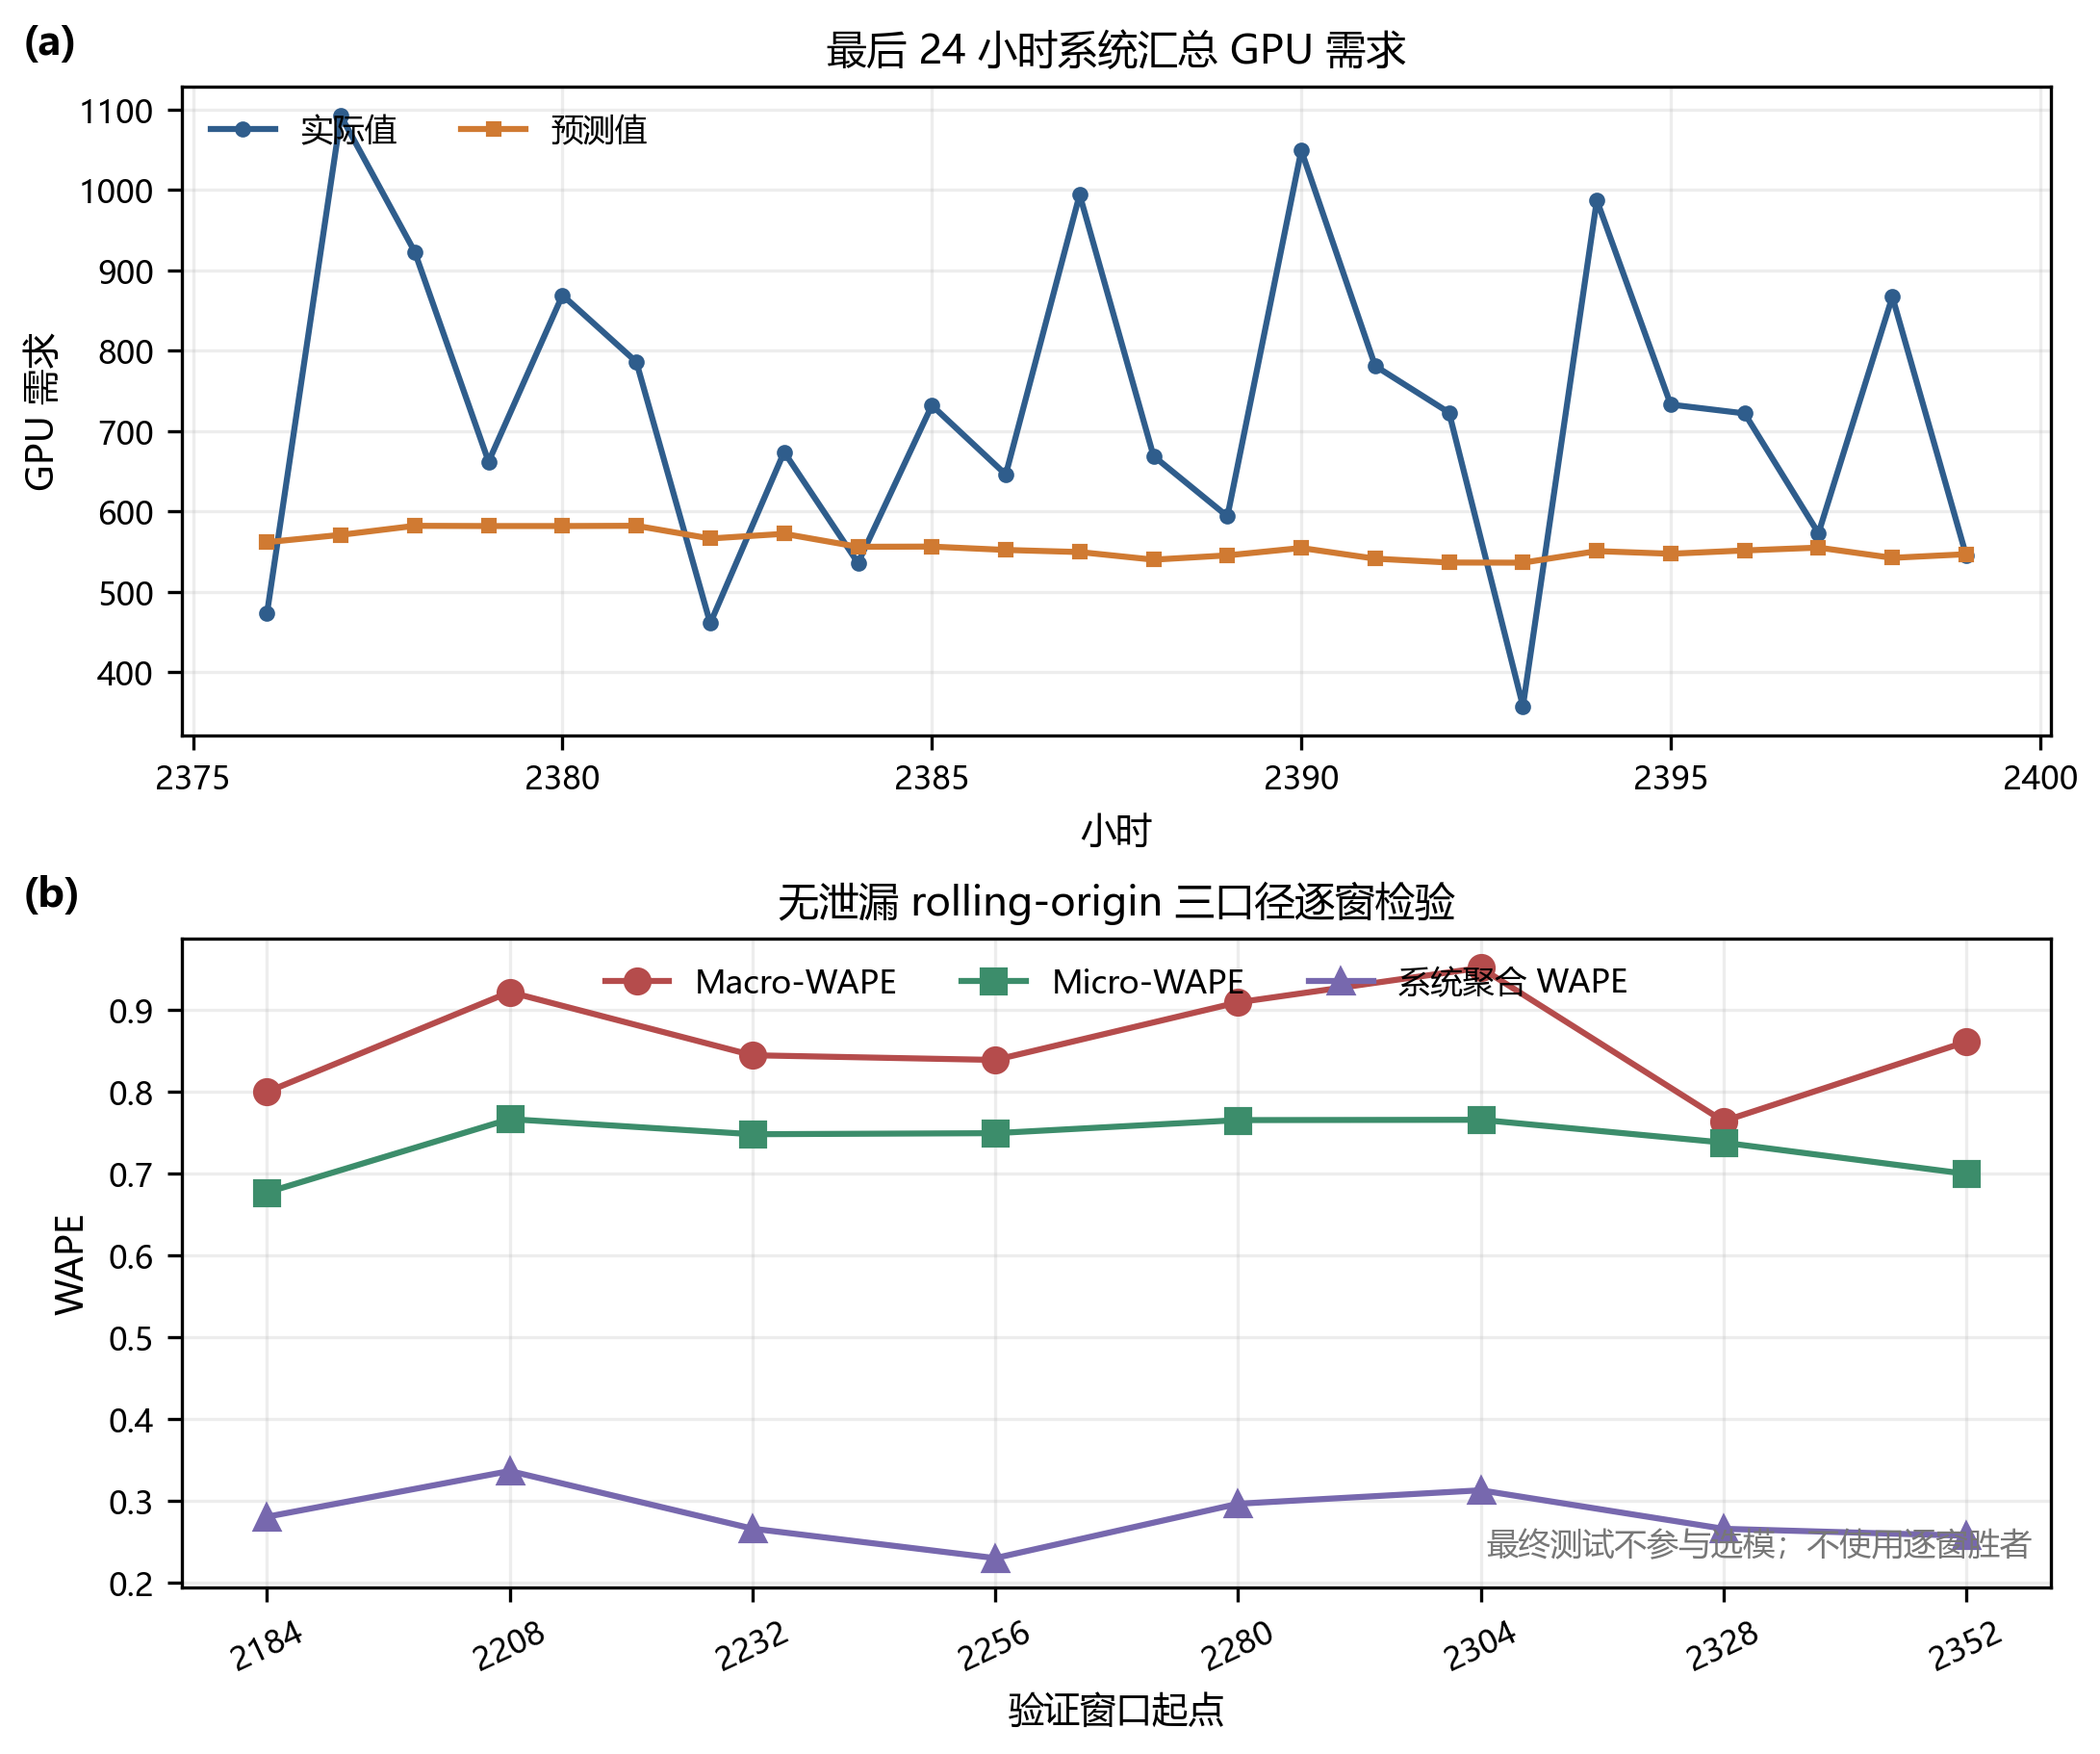
\includegraphics[width=.94\textwidth]{fig01_q1_forecast.png}
\caption{问题一预测效果：（a）第 2376--2399 小时系统汇总实际值与预测值；（b）无泄漏 rolling-origin 窗口的 Macro-WAPE、Micro-WAPE 和系统聚合 WAPE。三种口径均使用各序列按 8 窗口综合规则选定的候选，不使用逐窗胜者，最终测试不参与候选排序。}\label{fig:q1forecast}
\end{figure}

\subsubsection{538 个实际任务的独立末端调度}
预测只用于精度评价；基础调度读取全部 50000 个实际任务并保存独立 GPU 占用矩阵，随后筛选第 2376--2399 小时实际到达的 538 个任务形成题定调度表。该表与问题二 balanced 调度使用不同变量、不同 CSV 和不同 SHA-256 来源。完整 Q1 调度通过任务唯一性、到达与完成时限、单向网络时延、GPU、IT 功率和设施功率复算；其中 68 个末端任务在第 2400--2405 小时结清，第 2406 小时无任务占用。

问题一的区域--小时 GPU 利用率由完整基础调度在第 2376--2399 小时的实际占用直接重建，而非仅筛选到达时刻，也不引用问题二调度。六区域 24 小时的峰值利用率为 0.997036，算术平均为 0.490167。任务级实际起止时刻、执行区域、任务类型和区域利用率合并见图~\ref{fig:q1schedule}。图~\ref{fig:q1schedule}a 展示 538 个末端任务在六区域的连续执行区间，包含延伸至第 2405 小时的结清任务；图~\ref{fig:q1schedule}b 显示区域 E、F 在部分小时接近容量上限，而所有曲线均未越过 100\%，与正式容量审计一致。
\begin{figure}[H]\centering
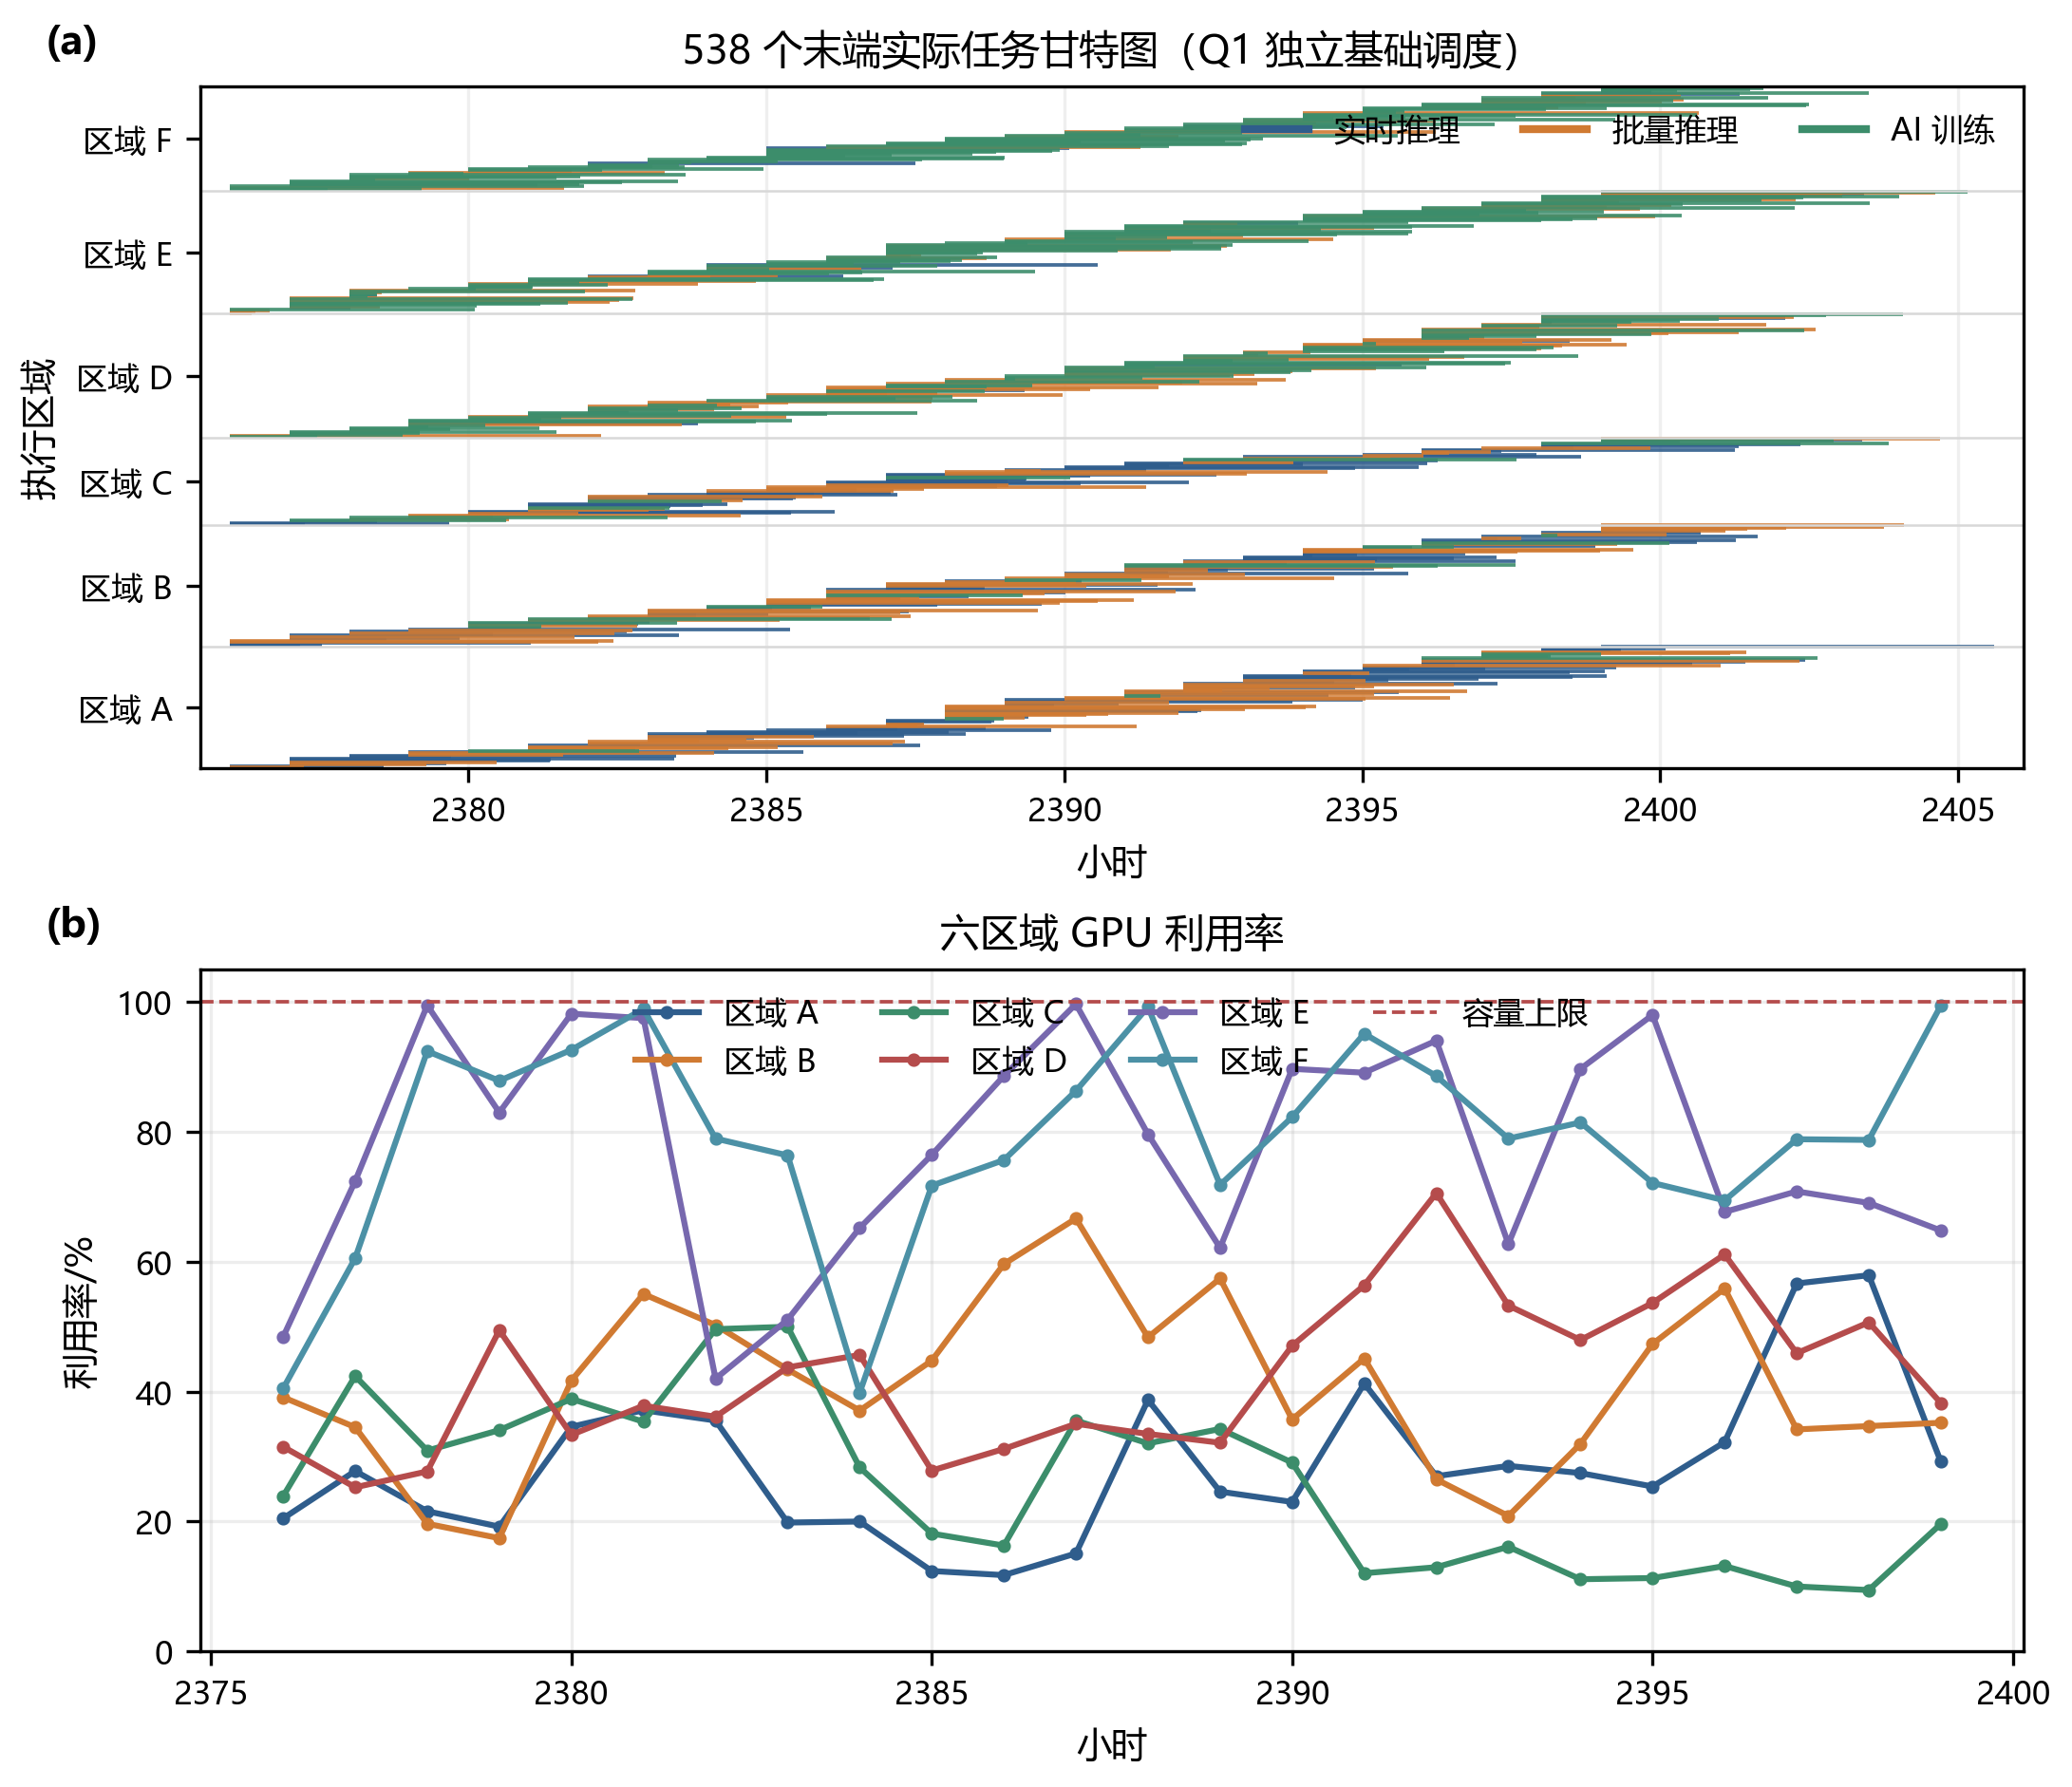
\includegraphics[width=.94\textwidth]{fig02_q1_schedule.png}
\caption{问题一独立基础调度结果：（a）538 个末端实际任务甘特图；（b）由 Q1 完整基础调度复算的六区域 GPU 利用率。两幅子图均未读取 Q2 schedule。}\label{fig:q1schedule}
\end{figure}

\subsection{问题二：公共候选流与四目标增量搜索}
问题二不启用储能。任务 $i$ 在小时 $t$ 的重叠长度为
\begin{equation}
\omega_{it}=\max\{0,\min(t+1,f_i)-\max(t,s_i)\}.
\end{equation}
若 $\omega_{it}>0$，其完整 GPU 与 IT 功率进入瞬时容量状态；结算电量则为 $p_i\omega_{it}$。因此
\begin{equation}
E^{AI}_{rt}=\sum_{i:r_i=r}p_i\omega_{it},\qquad
L^F_{rt}=\pi_r\bigl(E^{AI}_{rt}+E^{N}_{rt}\bigr)/1\mathrm h .
\end{equation}
该分离同时用于完整重算和候选增量，不能把 fractional-duration 任务的完整 $p_i$ 当作一小时电量。无储能能源满足
\begin{align}
R^{use}_{rt}&=\min\{R^{av}_{rt},L^F_{rt}\},\\
G^{buy}_{rt}+R^{use}_{rt}&=L^F_{rt},\\
R^{use}_{rt}+R^{sell}_{rt}+R^{curt}_{rt}&=R^{av}_{rt},
\end{align}
并满足购售电上限与互斥。

服务优化目标统一定义为 GPU-hour 加权的时延与等待：
\begin{equation}
J_s=\frac{\sum_i g_i(f_i-s_i)[\ell_i+10(s_i-a_i)]}{\sum_i g_i(f_i-s_i)},
\qquad Q_s=\frac{1}{1+J_s}.
\end{equation}
$J_s$ 是优化目标，$Q_s$ 只作同口径无量纲报告；网络时延、实时 SLA、按期率和等待分位是辅助解释指标。

五个 direct 方向均从同一 Q1 基线出发，共享目标无关的 120000 行 BaseCandidate 池及其顺序。语义键 $(TaskID,Region,CandidateStart)$ 全局唯一：第 1 层为 50000 个任务各自唯一的基线赋值，第 2 层含 49512 个有效替代，第 3 层含 20488 个有效替代；耗尽任务直接跳过，不复制末项。五方向各完成预声明的 6 个完整 pass。若完整一遍接受数为 0，或连续两遍同时满足主目标相对改善不超过 $10^{-3}$、接受率不超过 $10^{-3}$ 且硬约束与增量/全量重建审计通过，则判为声明邻域内稳定；非目标辅助指标只作诊断。

平衡评分不再拼接任意原始单位。对公共池中 115778 个基线可行候选，以 ideal--nadir 极差 $d_j$ 标准化增量：
\begin{equation}
\Psi=\tfrac14\left(\frac{\Delta C}{d_C}+\frac{\Delta E}{d_E}-\frac{\Delta R}{d_R}+\frac{\Delta J_s}{d_s}\right).
\end{equation}
四个尺度分别为 88972.8988 CNY、17.842975 tCO$_2$、329.404133 MWh 和 3.773375 服务单位，固定权重均为 0.25，参数在搜索前由公共池生成。

\begin{table}[H]\centering
{\small
\caption{问题二五方向在共同第 5 个完整 pass 的结果}\label{tab:q2schemes}
\begin{tabular}{lrrrrrr}\toprule
方向 & 成本/亿元 & 碳/t & 新能源率 & 服务目标 & 可行数 & 接受数\\\midrule
成本 & -4.402587 & 21.5756 & 0.686387 & 241.0299 & 281464 & 6354\\
直接碳 & -4.196800 & 0.0000 & 0.679085 & 5.1747 & 328675 & 18\\
新能源 & -4.394138 & 26.0817 & 0.686859 & 417.2252 & 259944 & 19809\\
服务 & -4.196583 & 14.3916 & 0.679078 & 5.1593 & 328890 & 2\\
平衡 & -4.393037 & 0.4275 & 0.686668 & 131.4759 & 273866 & 19182\\\bottomrule
\end{tabular}}
\end{table}

每个方向每遍完整检查 120000 个 BaseCandidate；任务检查覆盖率为 100\%，具有有效替代候选的任务覆盖率为 99.024\%。成本、直接碳、新能源、服务和平衡分别在第 4、2、4、2、5 遍满足预声明稳定条件，因此正式横向比较取最早共同完成的第 5 遍，即每方向累计 600000 次尝试。该 converged 仅表示主目标改善与接受率达到声明阈值，并非零接受固定点或全局最优。平衡方案用于 Q3/Q4 下游。直接碳从 Q1 基线开始并进入公平比较；额外 carbon multistart 从成本、平衡和直接碳三个正式末态出发，每个起点新增 20000 个候选，最终仍选中 carbon\_direct 起点且碳为 0，只作为强化实验，不替代直接碳行。

\begin{table}[H]\centering
{\small
\caption{问题二成本现金流分解}\label{tab:q2cost}
\begin{tabular}{lrrrrr}\toprule
方向 & 购电/MWh & 售电/MWh & 购电支出/万元 & 售电收入/亿元 & 净成本/亿元\\\midrule
成本 & 74.3386 & 1409164.6046 & 2.0112 & 4.402788 & -4.402587\\
直接碳 & 0.0000 & 1329621.3157 & 0.0000 & 4.196800 & -4.196800\\
新能源 & 72.5931 & 1407119.7303 & 2.3889 & 4.394377 & -4.394138\\
服务 & 40.4664 & 1329591.4740 & 1.2328 & 4.196706 & -4.196583\\
平衡 & 1.5264 & 1405896.3337 & 0.0397 & 4.393041 & -4.393037\\\bottomrule
\end{tabular}}
\end{table}
负成本主要来自题面售电收入边界，并不表示全生命周期成本为负。等权、成本偏置、碳偏置、新能源偏置和服务偏置五组权重下，现有五个 direct 末态的最低标准化分数均对应 formal balanced，Q4 基线未发生离散切换；这只说明本次有限方案集内没有轻微权重失稳。

图~\ref{fig:q2multi}a 把成本、碳排放和网络时延按“越小越优”，新能源利用率和服务质量按“越大越优”分别作方案间 min--max 同向化；该分数只用于可视化，表~\ref{tab:q2schemes} 的原始量纲指标保持不变。成本、新能源和服务方向分别突出其对应目标，formal balanced 在成本、碳和新能源利用率上较均衡，但服务质量并非最优。图~\ref{fig:q2multi}b 显示 balanced 的首轮改进和接受数最大，随后随累计候选数增加迅速下降；第 5 遍达到预声明阈值稳定，只能解释为有限候选邻域内收敛。
\begin{figure}[H]\centering
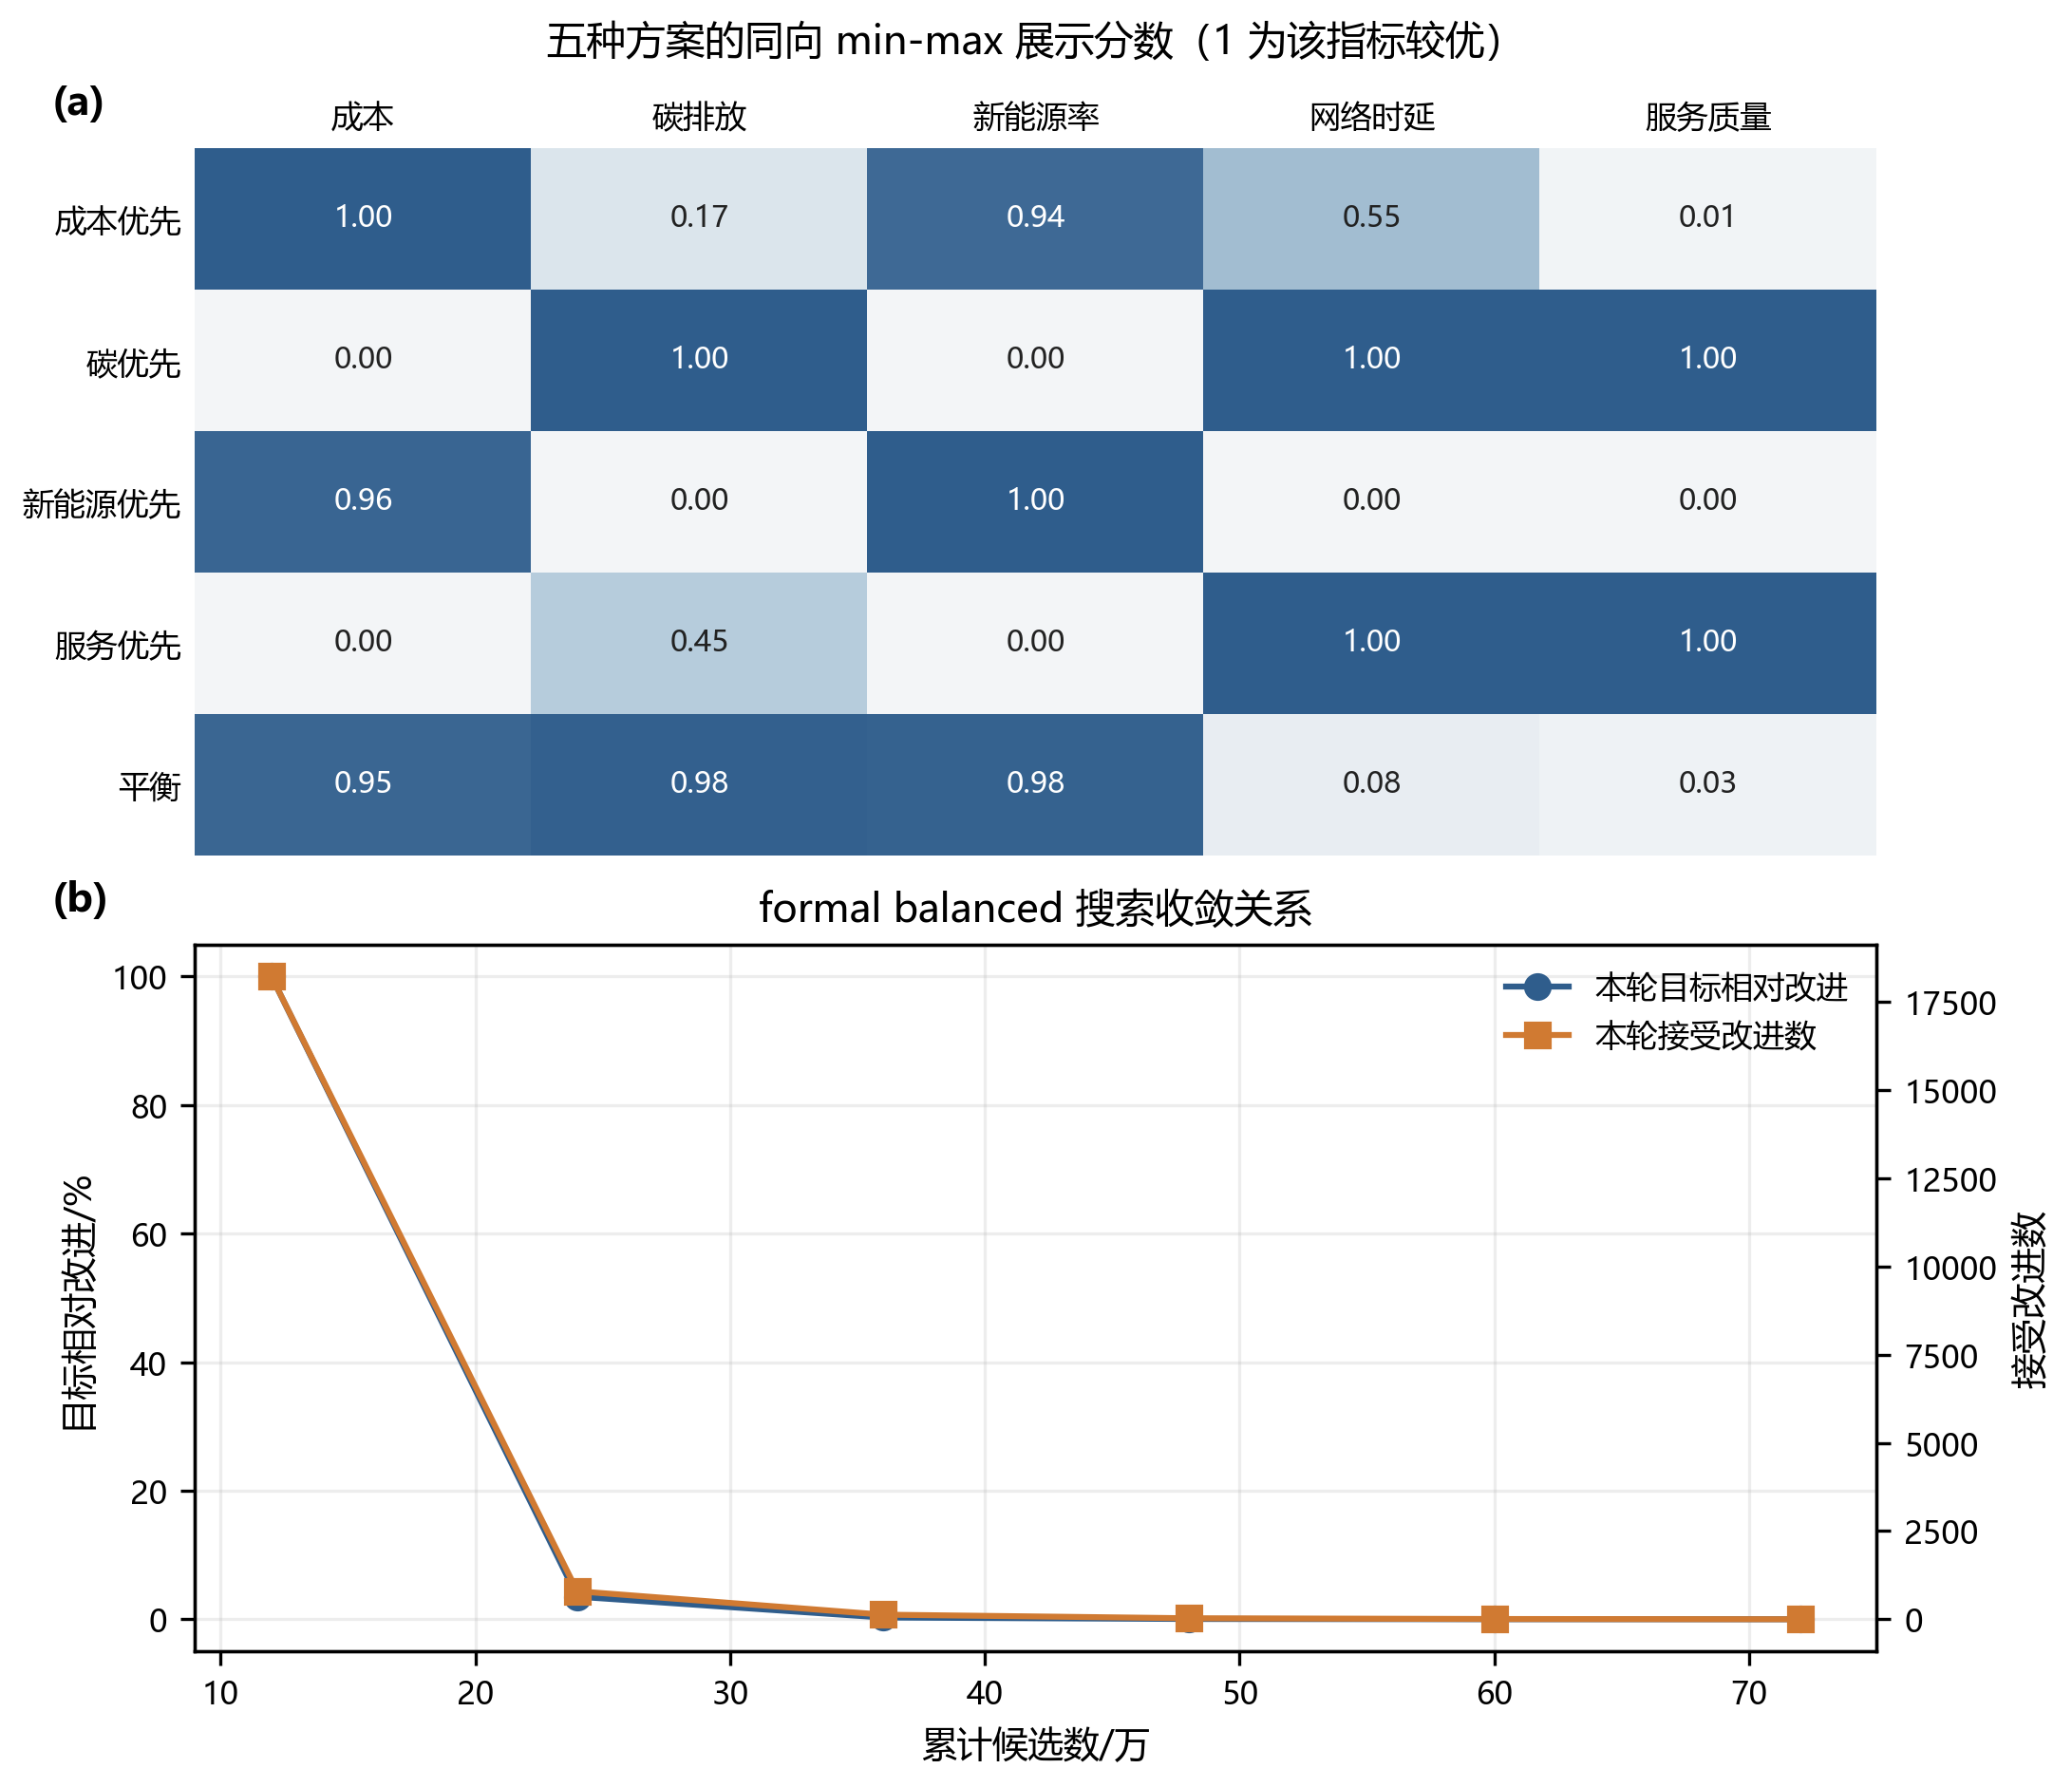
\includegraphics[width=.94\textwidth]{fig03_q2_multiobjective.png}
\caption{问题二有限候选邻域的多目标结果：（a）五种 direct 方案的同向 min--max 展示分数，1 表示该指标在五方案中较优；（b）formal balanced 的累计候选数、本轮目标相对改进和本轮接受改进数。}\label{fig:q2multi}
\end{figure}


\subsection{问题三模型建立：统一来源核算与净电网波动优化}
Q3 固定使用 Q2 formal balanced 调度按小时重建的设施负荷，不在本问重新改变任务执行区域或开工时刻；Q3/Q4 统一使用来源显式能源流。对每个区域小时，充放电和购售电分解为
\begin{align}
C_{rt}&=R^{ch}_{rt}+G^{ch}_{rt}, &D_{rt}&=D^{load}_{rt}+D^{sell}_{rt},\\
G^{buy}_{rt}&=G^{load}_{rt}+G^{ch}_{rt}, &G^{sell}_{rt}&=R^{sell}_{rt}+D^{sell}_{rt},\\
R^{av}_{rt}&=R^{direct}_{rt}+R^{ch}_{rt}+R^{sell}_{rt}+R^{curt}_{rt}.
\end{align}
\subsubsection{能源与储能约束}
逐区域逐小时满足能源平衡、储能 SOC 递推、容量与充放电功率边界；同一小时充电与放电互斥，购电与售电也互斥，终端 SOC 恢复至初始值。新能源依次直接供负荷、充储能、外送、弃电；网充和储能售电不计入新能源利用量，储能放电也不重复计量。因此
\begin{equation}
U_{RE}=\frac{\sum_{r,t}(R^{direct}_{rt}+R^{ch}_{rt}+R^{sell}_{rt})}{\sum_{r,t}R^{av}_{rt}}.
\end{equation}
定义 $N_{rt}=G^{buy}_{rt}-G^{sell}_{rt}$，则 $P_{peak}=\sum_r\max_t\max(N_{rt},0)$，正式净波动为
\begin{equation}
V=\sum_r\sum_{t=1}^{2406}|N_{rt}-N_{r,t-1}|,
\end{equation}
不虚构 $t=-1$。真正的净波动策略以相邻 SOC 对 $(S_{r,t-1},S_{rt})$ 为边状态，保存该边的 $N_{rt}$，下一步精确累加相邻绝对差；21 状态下每区复杂度为 $O(TK^3)$、内存为 $O(TK^2)$。小型离散样例与穷举最优一致，且购电恒零、售电波动的反例会得到非零 $V$。

内部吞吐与等效完整循环采用
\begin{equation}
Q_r=\sum_t(\eta_r^cC_{rt}+D_{rt}/\eta_r^d),\qquad EFC_r=\frac{Q_r}{2(S_r^{max}-S_r^{min})},\quad EFC=\sum_rEFC_r,
\end{equation}
其中所有区域均满足 $S_r^{max}>S_r^{min}$。

\begin{table}[H]\centering\scriptsize
\caption{问题三七策略的修正后指标}\label{tab:q3policies}
\resizebox{\textwidth}{!}{\begin{tabular}{lrrrrrr}\toprule
策略 & 成本/亿元 & 碳/t & 新能源率 & 净购电峰值/MW & 净波动/MW & EFC\\\midrule
no-action & -4.393037 & 0.4275 & 0.686668 & 1.5264 & 58044.0 & 0.000\\
成本 & -4.541971 & 0.0000 & 0.693120 & 0.0000 & 22178.7 & 92.227\\
碳 & -4.394658 & 0.0000 & 0.686743 & 0.0000 & 57727.3 & 1.218\\
新能源 & -4.541576 & 0.0000 & 0.693131 & 0.0000 & 22331.9 & 92.451\\
峰值 & -4.394658 & 0.0000 & 0.686743 & 0.0000 & 57727.3 & 1.218\\
净波动 & -4.525500 & 0.0000 & 0.692492 & 0.0000 & 17586.8 & 85.045\\
平衡 & -4.541740 & 0.0000 & 0.693131 & 0.0000 & 22150.2 & 92.401\\
\bottomrule\end{tabular}}
\end{table}
修正后不重复非支配候选为成本、净波动和平衡策略，其理想点距离分别为 0.387360、0.670820 和 0.384975，故正式策略由原成本策略改为平衡策略，而非按名称预设。所选方案成本为 $-4.541740\times10^8$ 元，新能源利用率为 0.693131，净波动为 22150.241 MW，EFC 为 92.401。其新能源直接利用、充电和外送分别为 6525650.592、74699.362 和 1405847.711 MWh；网充为 0，储能售电为 65300.656 MWh。最大总能源平衡残差和来源分解残差分别为 $5.68\times10^{-14}$ MW 与 $1.42\times10^{-14}$ MW。
图~\ref{fig:q3storage}a 的无储能基准直接读取正式字段 $N_{rt}=G_{rt}^{buy}-G_{rt}^{sell}$，没有反推或构造数据；储能使系统净电网功率整体下移。图~\ref{fig:q3storage}b 给出六区域 SOC 的逐时轨迹，均受容量与终端等式约束；图~\ref{fig:q3storage}c 表明无储能时仅区域 F 出现 1.5264 MW 的非负峰值净购电，所选策略将其降至 0。图~\ref{fig:q3storage}d 以无储能为分母同向计算相对改善，净波动由 58043.980 MW 降至 22150.241 MW，峰值消除，弃电量亦有小幅下降；这些百分比只作展示，原始指标仍以表~\ref{tab:q3policies} 为准。
\begin{figure}[H]\centering
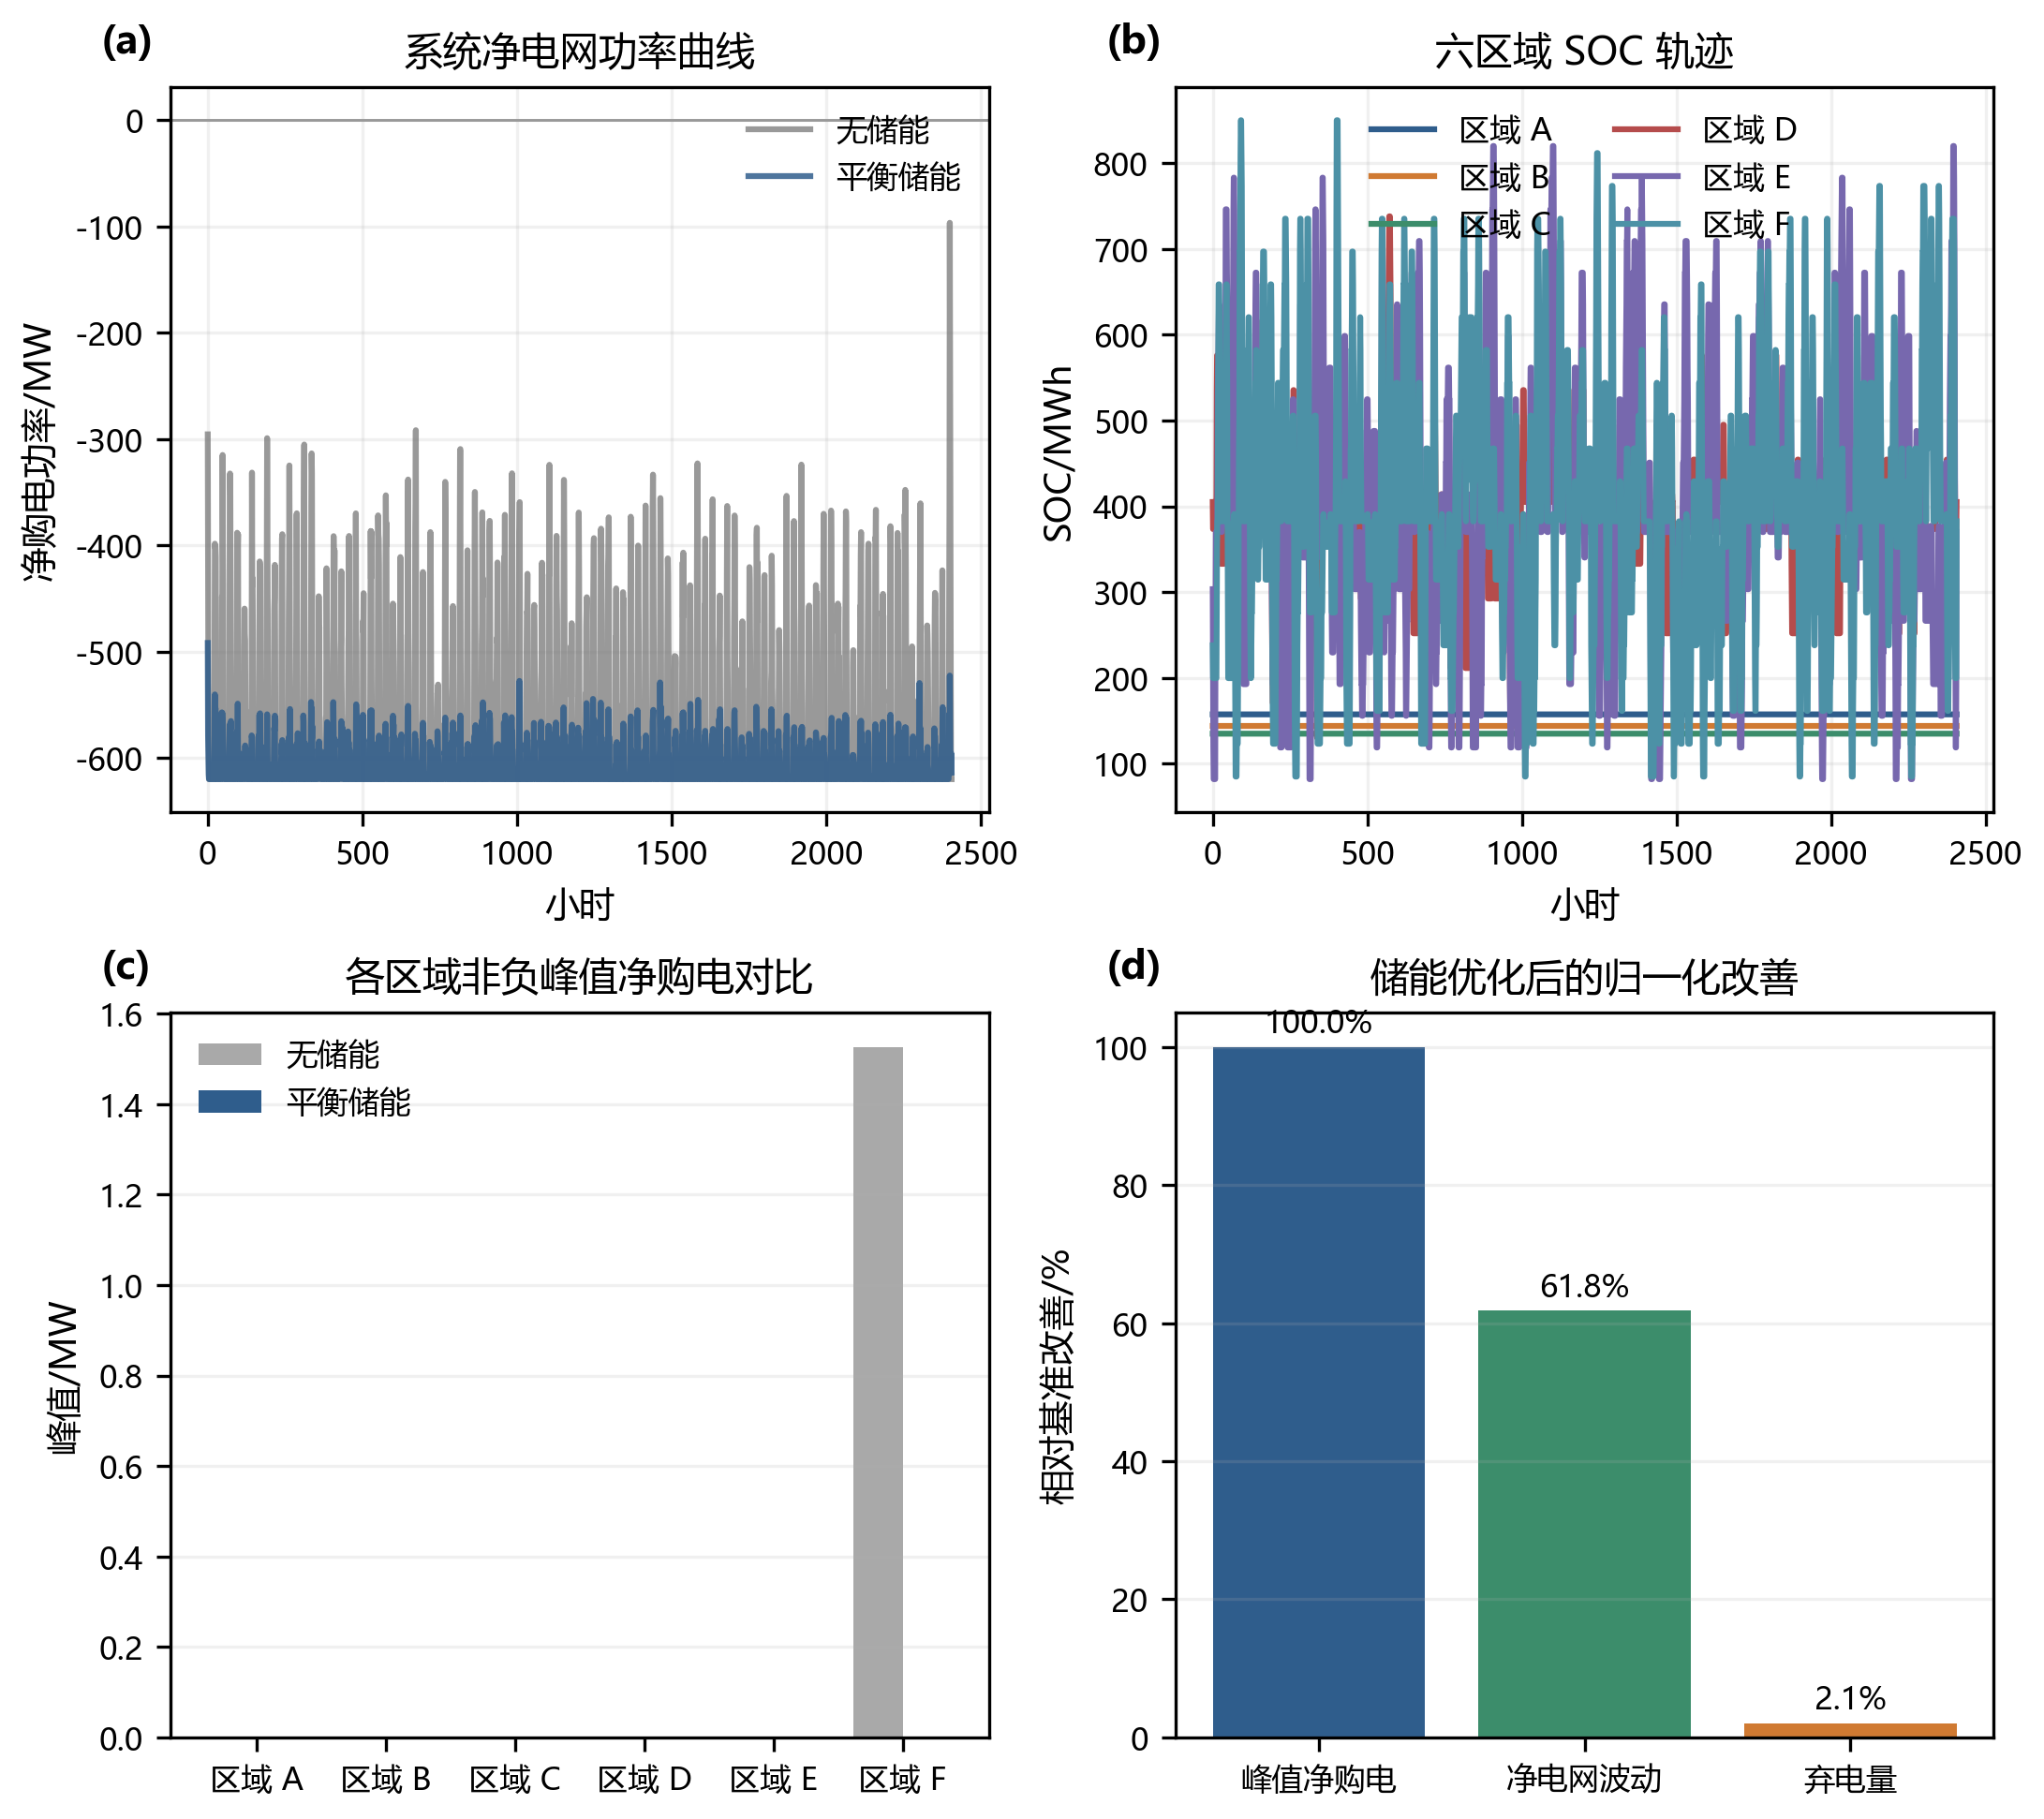
\includegraphics[width=.96\textwidth]{fig04_q3_storage.png}
\caption{问题三储能优化结果：（a）无储能与所选平衡储能的系统净电网功率；（b）六区域 SOC；（c）各区域非负峰值净购电；（d）峰值、净波动与弃电量相对无储能基准的改善。}\label{fig:q3storage}
\end{figure}
图数据全部绑定 solve v19 的 Q3 正式逐时流与审计表；本次 Q4 联合基准虽选择同一储能轨迹，Q3 子图仍不读取 Q4 文件。

\subsection{问题四：嵌套碳候选银行与 17 情景重算}
\subsubsection{问题四情景设计}
每个情景只改变其声明因素，其余任务集、设备容量、网络时延、功率映射和评价公式保持不变，并从共同基线独立重启。

Q4 继续绑定 formal balanced 任务调度哈希，全部情景统一使用 21 个 SOC 状态，并调用与 Q3 相同的来源分解、$U_{RE}$、净峰值、净波动、EFC 和硬约束审计。任务候选的 \texttt{SearchSignal} 由正式电价、碳强度、购电和弃电组成；正式成本始终用未被覆盖的 \path{ElectricityPrice_CNY_per_MWh} 结算。

碳削减 0、10\%、20\%、30\% 按由松到严求解。每档候选银行含正常联合基准、当前交替搜索候选、三种储能政策和全部较松档候选，并在当前档输入上重新核算。四档目标依次为 7430.328、6687.295、5944.262、5201.229 tCO$_2$；候选数为 6、9、12、15。前两档分别找到 5、6 个可行候选；后两档在声明搜索内未找到达标候选，记为 \path{target_not_found_within_declared_search}，不解释为数学不可行。

\begin{table}[H]\centering\scriptsize
\caption{问题四全部 17 个情景的核心指标}\label{tab:q4scenarios}
\resizebox{\textwidth}{!}{\begin{tabular}{lrrrrrr}\toprule
情景 & 成本/亿元 & 碳/t & 时延/ms & 服务质量 & 新能源率 & 净购电峰值/MW\\\midrule
基准 & -4.541740 & 0.00 & 16.999 & 0.007549 & 0.693131 & 0.00\\
碳减排 0.00 & -4.085543 & 6597.84 & 17.474 & 0.006447 & 0.849337 & 102.32\\
碳减排 0.10 & -4.089528 & 6489.85 & 17.526 & 0.006430 & 0.849420 & 106.90\\
碳减排 0.20 & -4.088342 & 6520.11 & 17.466 & 0.006374 & 0.849360 & 112.13\\
碳减排 0.30 & -4.084323 & 6751.80 & 17.534 & 0.006441 & 0.849313 & 112.30\\
价差 0.75 & -4.541740 & 0.00 & 16.999 & 0.007549 & 0.693131 & 0.00\\
价差 1.00 & -4.542140 & 0.00 & 17.046 & 0.007534 & 0.693149 & 0.00\\
价差 1.25 & -4.541740 & 0.00 & 16.999 & 0.007549 & 0.693131 & 0.00\\
售电 0.00 & 0.000000 & 0.00 & 17.051 & 0.007538 & 0.693146 & 0.00\\
售电 0.50 & -2.270870 & 0.00 & 16.999 & 0.007549 & 0.693131 & 0.00\\
售电 1.00 & -4.541740 & 0.00 & 16.999 & 0.007549 & 0.693131 & 0.00\\
新能源 0.80 & -4.092708 & 6473.67 & 17.514 & 0.006199 & 0.849435 & 205.98\\
新能源 1.00 & -4.541740 & 0.00 & 16.999 & 0.007549 & 0.693131 & 0.00\\
新能源 1.20 & -4.591580 & 0.00 & 16.999 & 0.007549 & 0.578413 & 0.00\\
波动 2026 & -4.519460 & 1695.10 & 17.600 & 0.006682 & 0.693534 & 294.79\\
波动 2027 & -4.515634 & 1716.07 & 17.659 & 0.006830 & 0.693363 & 320.78\\
波动 2028 & -4.519042 & 1351.78 & 17.606 & 0.006872 & 0.693504 & 241.90\\
\bottomrule\end{tabular}}
\end{table}
正常基准与 joint baseline 在成本、碳、新能源率、净峰值和净波动上逐项一致；网络时延为 16.998674 ms、服务质量为 0.007549。等待、实时 SLA、按期率、净波动和逐时能源流完整保存在结构化情景表及逐时表中。低新能源与三组波动种子使碳排和峰值显著上升，说明这些结论依赖题面情景，而非部署层鲁棒保证。

图~\ref{fig:q4scenarios}a 表明 10\% 碳削减目标在声明搜索内找到达标候选，而 20\% 和 30\% 点以叉号标示 \texttt{target\_not\_found\_within\_declared\_search}，不能按普通最优点解释；0\% 点机制未激活，使用空心标记。图~\ref{fig:q4scenarios}b 的三个峰谷系数均为 \texttt{mechanism\_active=false}，故只呈现为灰色空心点，不据此宣称价格机制有效。图~\ref{fig:q4scenarios}c 显示新能源系数降至 0.8 时购电量和碳排放重新出现，而系数 1.0 是未扰动参照。图~\ref{fig:q4scenarios}d 对联合基准、低新能源和波动种子 2027 作同向 min--max 展示；低碳、低峰值、低波动取反向标准化，高新能源率和高服务质量取正向标准化。所有情景仍是 scenario-feasible。
\begin{figure}[H]\centering
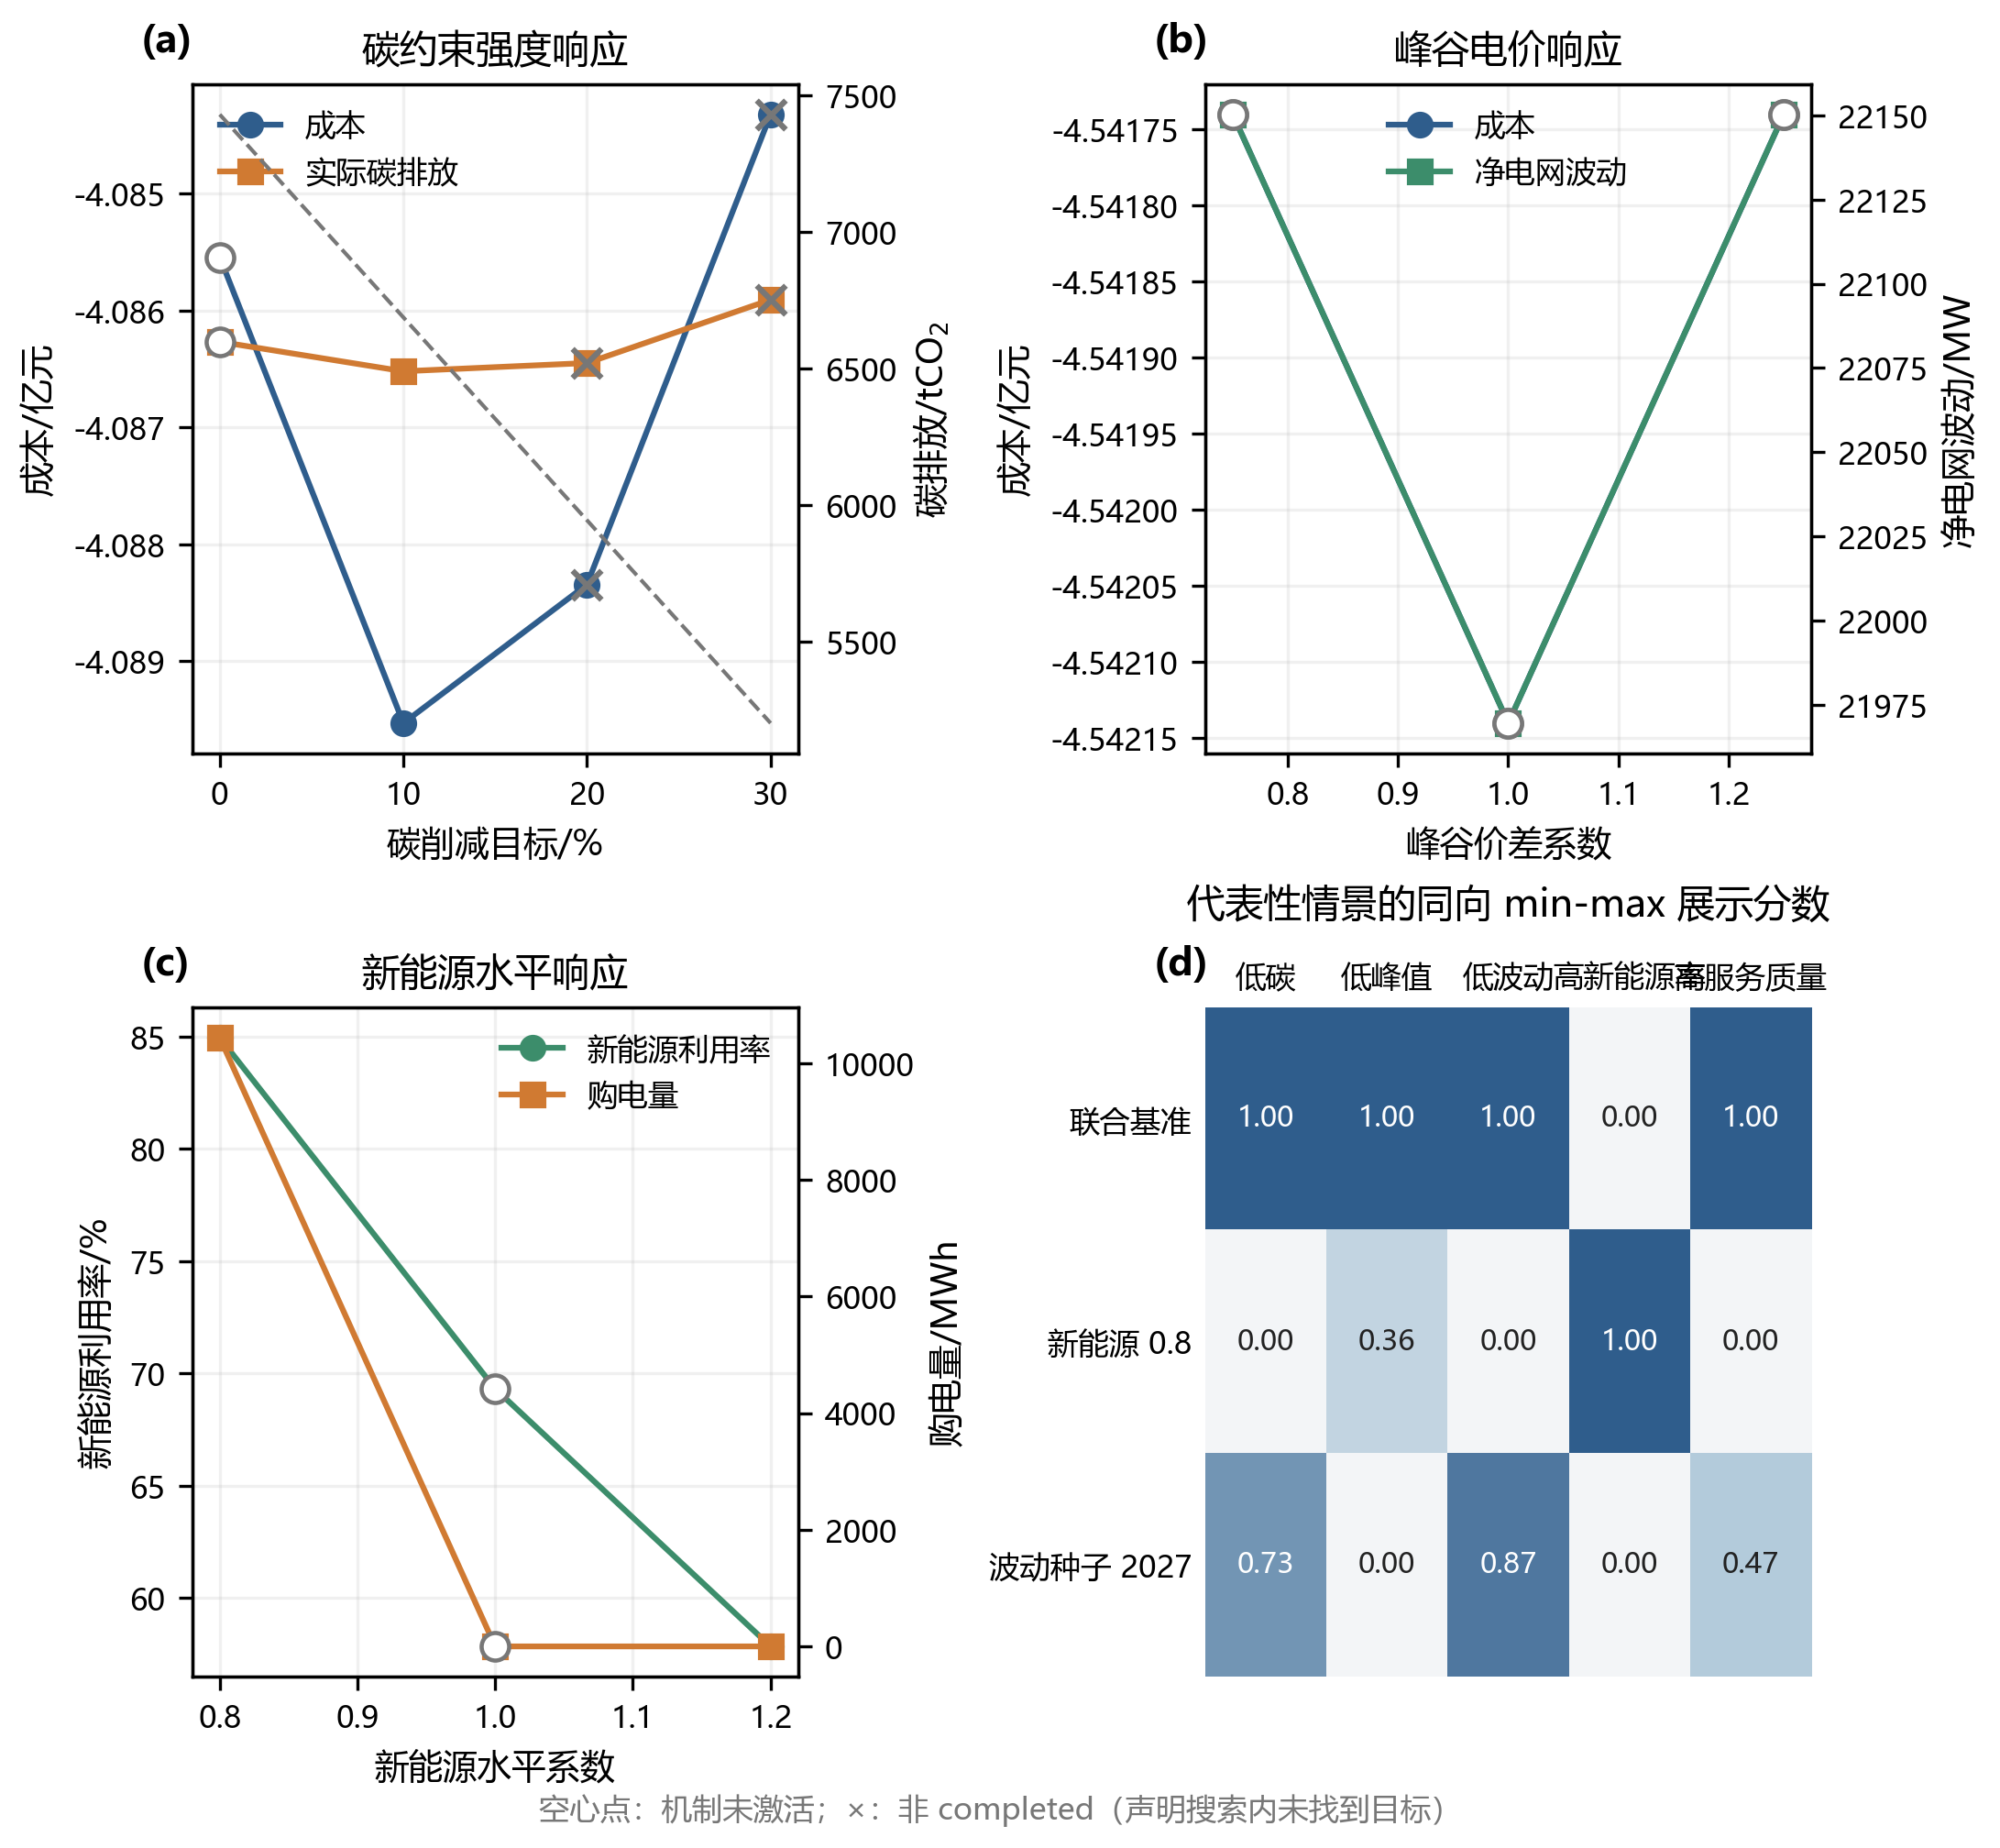
\includegraphics[width=.96\textwidth]{fig05_q4_scenarios.png}
\caption{问题四情景分析：（a）碳约束强度下的成本、实际碳排放与目标；（b）峰谷价差下的成本与净电网波动；（c）新能源水平下的利用率与购电量；（d）代表性情景的同向 min--max 展示分数。空心点表示机制未激活，叉号表示非普通 completed 状态。}\label{fig:q4scenarios}
\end{figure}

\subsection{方法边界}
% MMW-LIMITATION: D1
\paragraph{实现边界 D1}Q2 与 Q4 是预声明候选预算内的 best-found 可行解，不是穷举最优解。
% MMW-LIMITATION: D2
\paragraph{实现边界 D2}Q3 使用 21 个 SOC 网格状态，未计题面未给出的退化成本与循环寿命上限。
% MMW-LIMITATION: D3
\paragraph{实现边界 D3}Q4 的随机波动只使用固定种子 2026、2027、2028，并逐情景独立重启。
% MMW-LIMITATION: L1
\paragraph{证据边界 L1}无独立 Oracle，最高可信等级为 scenario-feasible。
% MMW-LIMITATION: L2
\paragraph{证据边界 L2}候选集内非支配不等于完整决策空间的 Pareto 前沿。
% MMW-LIMITATION: L3
\paragraph{证据边界 L3}Q2 方案名表示搜索方向，不表示跨方案的对应目标最小值。
\section{模型检验与灵敏度分析}

\subsection{统一约束审计与双运行检验}
任务审计逐项检查唯一执行、实时即时开工、到达、截止、单向网络时延、第 2406 小时禁占用、GPU、IT 和设施功率。能源审计统一检查
\begin{align}
e^{energy}_{rt}&=G^{buy}_{rt}+R^{av}_{rt}+D_{rt}-L^F_{rt}-C_{rt}-G^{sell}_{rt}-R^{curt}_{rt},\\
e^{SOC}_{rt}&=S_{rt}-S_{r,t-1}-\eta_r^cC_{rt}+D_{rt}/\eta_r^d.
\end{align}
此外逐行复核五个来源分解恒等式、$N_{rt}=G^{buy}_{rt}-G^{sell}_{rt}$、购售电与充放电互斥、功率边界和终端 SOC 等式。solve v19 中任务容量审计的最大正残差为 $1.364\times10^{-12}$；Q2 能源重算最大绝对残差为 $1.695\times10^{-11}$；Q3 与 Q4 的能源平衡和来源分解最大绝对残差分别为 $5.684\times10^{-14}$ MW 与 $1.421\times10^{-14}$ MW，其余 SOC、互斥、净购电恒等式和终端残差均为 0。

五方向 6 遍共形成 30 个累计状态检查点。候选级确定性分层审计共 430 个样本，覆盖 6 个 pass、accepted、feasible-but-rejected、capacity-rejected、no-change、fractional-duration、跨 2399/2400、返回基线、高功率与高 GPU 等类别；最大绝对和相对残差分别为 $8.009\times10^{-8}$ 和 $2.208\times10^{-9}$。公共候选池的 CandidateID 与语义三元组均唯一，全部 50000 个任务被检查，具有有效替代候选的任务覆盖率为 99.024\%。

两次完整正式复算已在本次论文修订之前由 code v21 完成，自然耗时分别为 4558.731 s 和 3786.555 s，均未设置显式墙钟上限。两次的 code SHA-256 均为 \texttt{1c777886...a6b71}，\texttt{results.json} SHA-256 均为 \texttt{c63996f2...9389e}；比较 106 份文件后结构化语义差异为 0。本次 paper-only 修订不再次运行 Q1--Q4 求解。

\subsection{问题二完整邻域多遍稳定性}
120000 行基础候选池的 BaseCandidateID 与由 TaskID、Region、CandidateStart 组成的语义三元组均 100\% 唯一。每个方向每遍按相同顺序完成 120000 次尝试；成本、直接碳、新能源、服务和平衡分别在第 4、2、4、2、5 遍达到预声明的主目标改善与接受率阈值，故正式共同完成点为第 5 遍。第 6 遍成本和平衡仍分别接受 4 和 1 个极小改善，说明此处“converged”是有限候选邻域的阈值稳定，不是零接受固定点或全局最优。

\subsection{统一参数灵敏度}
平衡方案基准成本为 $-4.393037\times10^8$ 元，直接购电量为 1.5264 MWh。购电价格整体缩放到 0.8、0.9、1.1、1.2 时，净成本分别为 $-4.393038$、$-4.393037$、$-4.393037$、$-4.393036$ 亿元；相对基准只变化约 $-79.37$ 至 $79.37$ 元，反映当前接近零购电边界，而非一般意义上的价格不敏感。新能源水平系数为 0.8、0.9、1.1、1.2 时，成本分别为 $-3.169013$、$-3.998509$、$-4.544149$、$-4.588926$ 亿元；新能源下降时购电缺口扩大，上升时外送上限与弃电约束削弱边际收益。

图~\ref{fig:sensitivity}a 采用“相对基准成本变化/元”避免用亿元坐标掩盖价格扰动的微小响应；图~\ref{fig:sensitivity}b 保留新能源扰动下的原始净成本量纲。两幅图只复算正式灵敏度 CSV 中已给出的目标值，不重新优化调度；它们与图~\ref{fig:q4scenarios}的联合情景分析口径不同，前者检验 Q2 固定方案参数响应，后者检验 Q4 联合任务--储能情景。
\begin{figure}[H]\centering
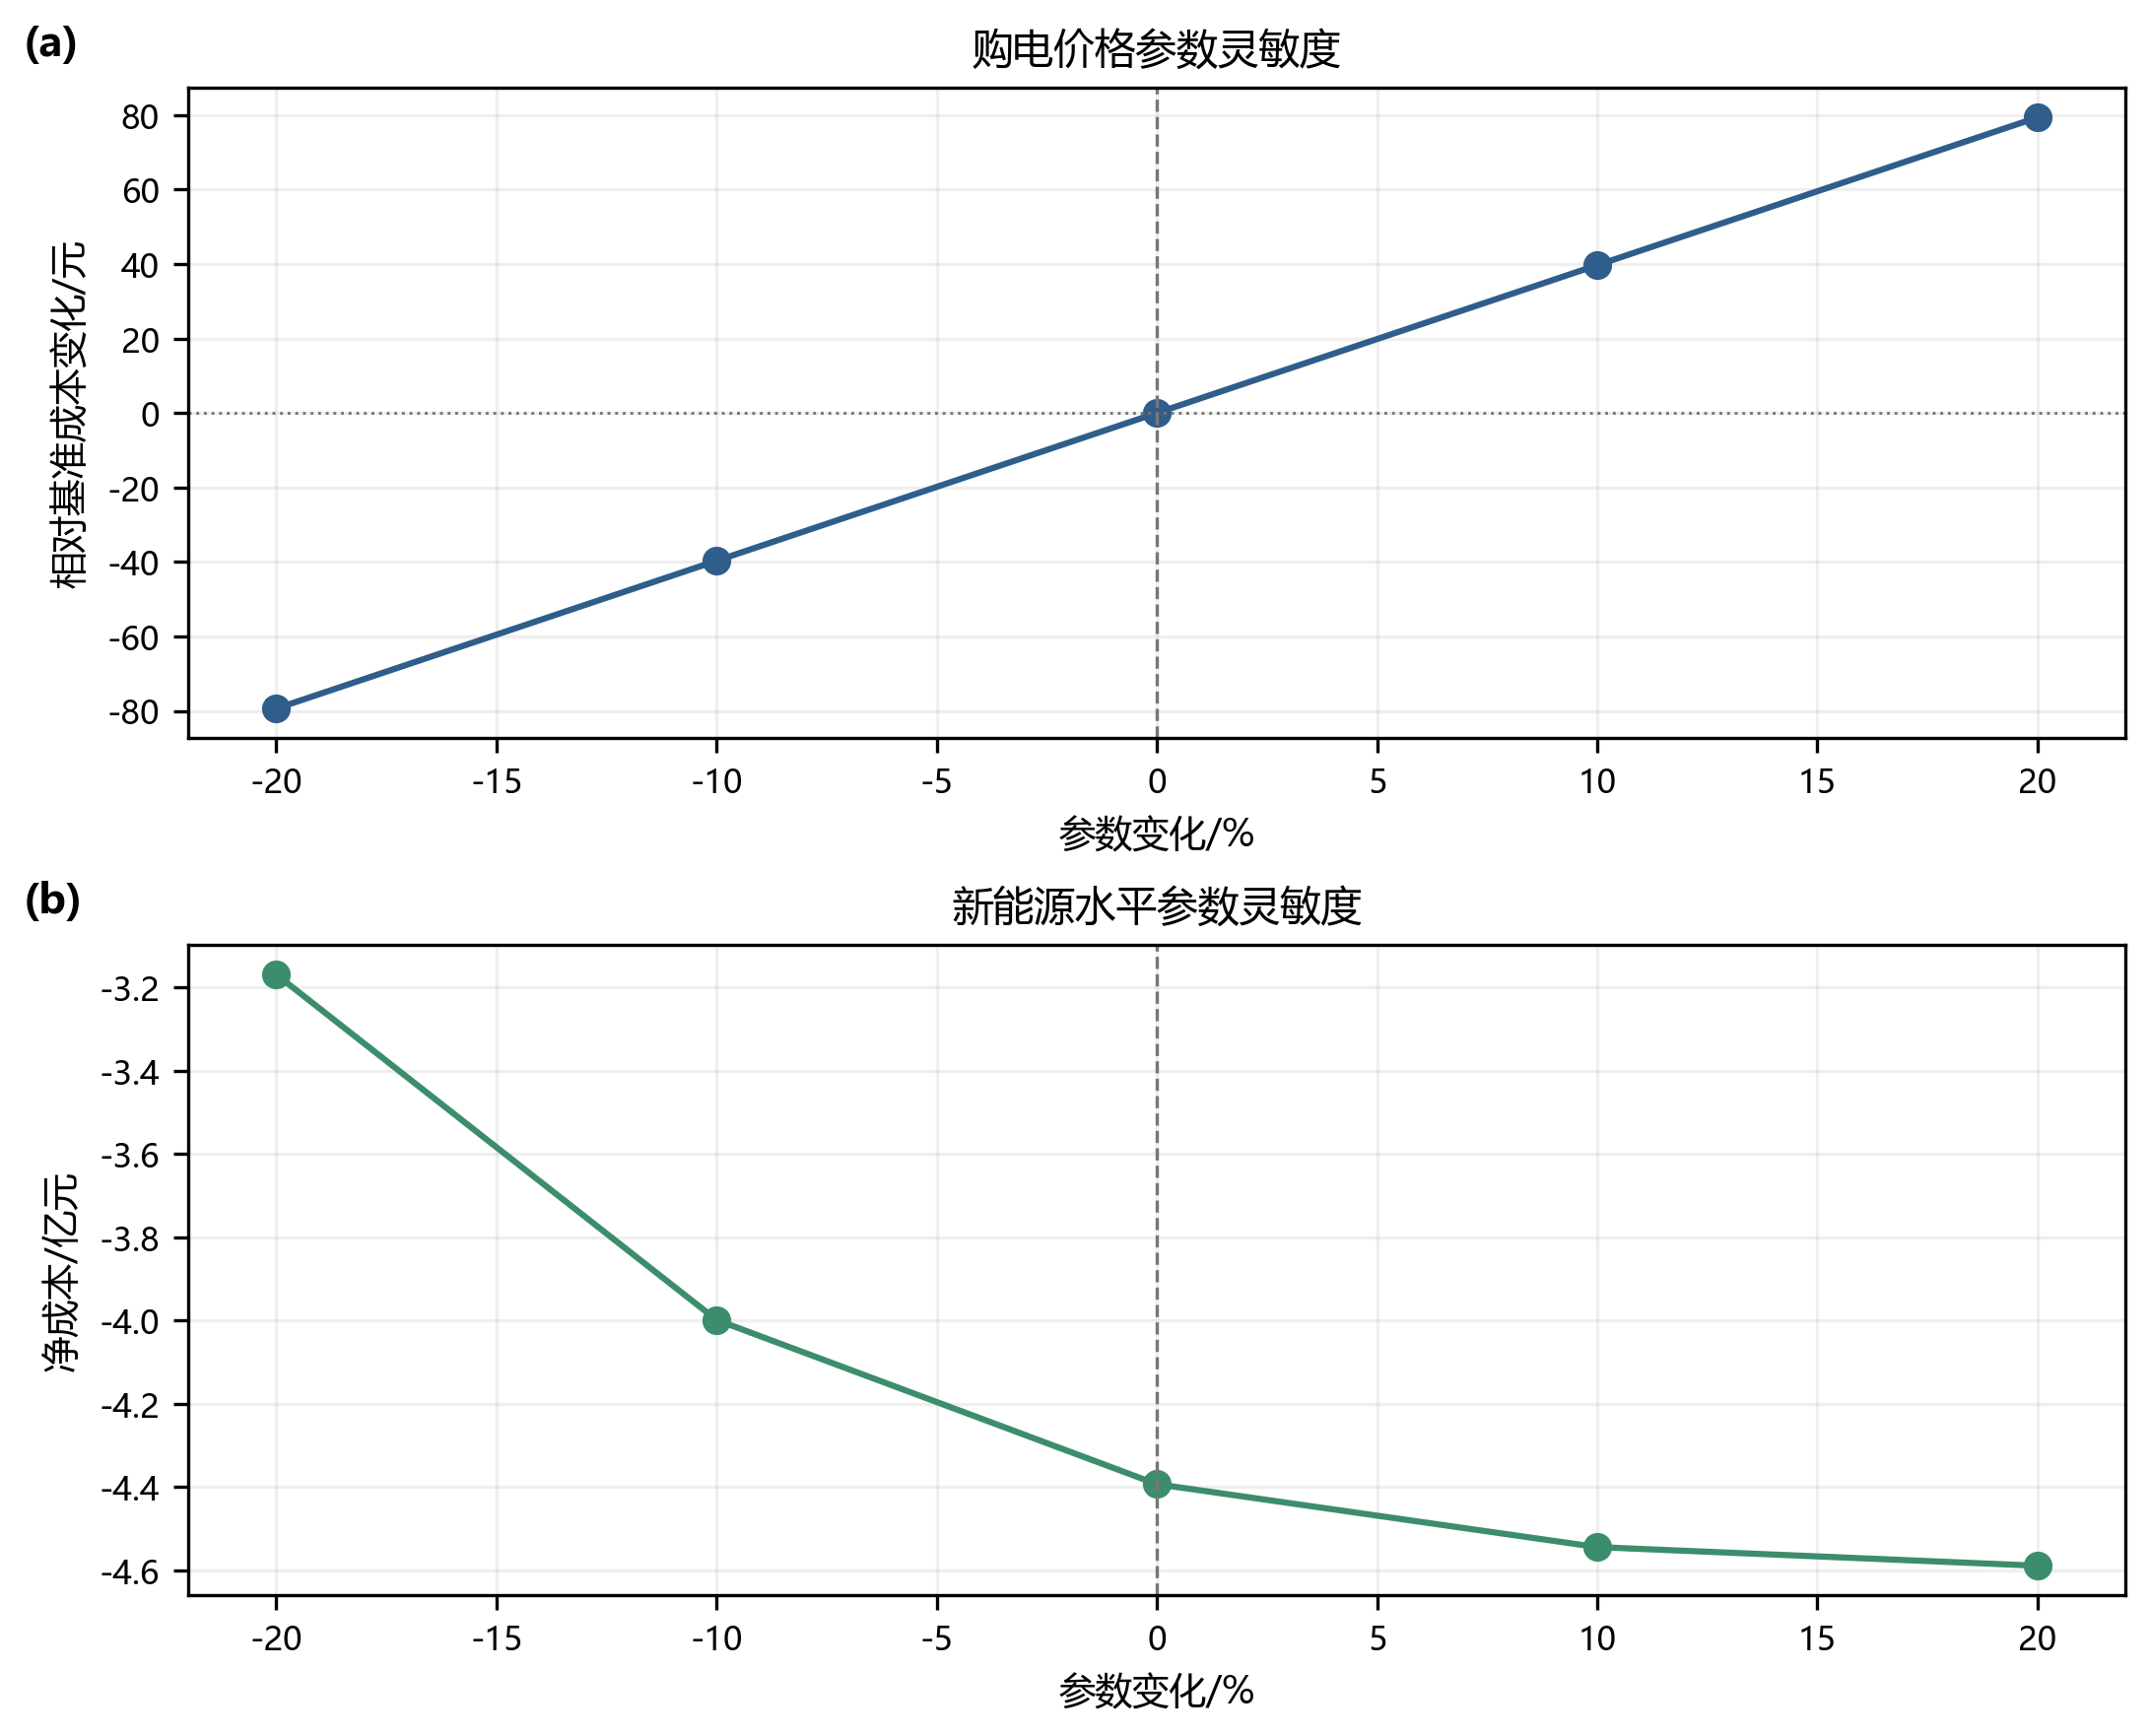
\includegraphics[width=.94\textwidth]{fig06_sensitivity.png}
\caption{统一参数灵敏度：（a）购电价格变化下相对基准的成本变化；（b）新能源水平变化下的净成本。}\label{fig:sensitivity}
\end{figure}

\subsection{SOC 网格与波动情景}
15、21、31 个 SOC 状态下，所选平衡策略成本分别为 $-4.528843$、$-4.541740$、$-4.559475$ 亿元；21 相对 31 状态的成本与新能源利用率相对误差分别为 0.38898\% 和 0.07163\%，三组最大约束残差均不超过 $5.684\times10^{-14}$。对应等效完整循环为 84.604、92.401、102.615。题面未给退化成本和循环上限，故只作为理想设备网格敏感性。

Q4 三个新能源波动种子的峰值购电为 241.896 至 320.783 MW、碳排放为 1351.780 至 1716.071 tCO$_2$，显示单一随机轨迹不足以概括风险；当前三种子只提供方向性稳健性证据，不能提升 scenario-feasible 可信等级。
\section{模型评价与推广}
\subsection{模型优点}
模型显式分离瞬时容量状态与小时重叠电量，避免 fractional-duration 任务被按整小时结算。Q1 的预测、基础调度及图形来源保持独立；Q2 五个 direct 方向共享语义唯一的 BaseCandidate 池与 6 遍相同顺序，直接碳与多起点强化分离，平衡评分使用公共 ideal--nadir 尺度；Q3/Q4 通过哈希绑定 formal balanced 下游输入，并共享来源显式能源流、净电网指标和可用 SOC 区间 EFC。增量/完整重算、全量硬约束、负向篡改、双运行和包清单共同构成可复核证据链。

五个 direct 方向均覆盖 50000 个任务，七个 Q3 策略和 17 个 Q4 情景均有逐行结构化结果。双运行确定性 bundle 哈希一致，故当前结果达到无独立 Oracle 条件下的 scenario-feasible 可信等级。

\subsection{模型不足}
Q2 已在共同第 5 遍达到预声明的主目标/接受率阈值稳定，但第 6 遍成本和平衡仍分别接受 4 和 1 个极小改善，且每任务最多只有三个基础候选；因此它不是零接受固定点，更没有全局最优证书。Q4 每轮只检查 600 个候选并最多 8 轮，同样只是有限预算 best-found。Q3 的 21 状态 SOC 也只给出网格内候选。储能未计退化、自放电和备用容量；所选方案 EFC 为 92.401，仍不能把账面收益直接解释为可部署收益。

通信侧只使用静态单向时延，未纳入带宽、拥塞和迁移能耗。formal balanced 的服务目标为 131.4759、服务质量为 0.007549，最大等待达到 1926 小时，说明综合评分没有消除尾部服务风险。Q4 正常联合基准购电碳为 0；在新能源短缺压力参照下，0\% 和 10\% 档找到达标候选，20\% 和 30\% 档只是在声明候选银行内未找到达标轨迹，并非数学不可行。负成本同样主要来自题面售电边界。

\subsection{问题一的鲁棒性与可追溯性}
题面单窗口切分被保留，并以 8 个完全位于最终测试之前的 expanding-window 原点检查时间稳定性。最终测试三种 WAPE 可由 432 条预测逐项复算，8 个滚动窗口的三口径曲线可由 3456 条选定候选逐小时预测复算；\texttt{schedule\_provenance.json} 绑定 Q1 全量表、538 条末端表、Q2 balanced 表及两张 Q1 图。负向替换测试会在 Q1/Q2 哈希同源或 provenance 漂移时失败。

System Aggregate WAPE 明显低于 Macro 与 Micro，部分来自序列间误差抵消，不能解释单序列容量风险。Q1 调度虽通过全时域审计，仍是确定性贪心的 scenario-feasible incumbent。

\subsection{推广方向}
后续应扩大 Q2 每任务时空邻域、比较零接受停止与阈值停止，并引入混合整数规划上下界，并继续使用同一公共候选与全量审计。Q3 可加入每 MWh 吞吐退化成本和年度循环上限；在线部署可采用滚动时域并传递绝对 SOC。多目标部分可用 $\varepsilon$-约束法扩充非支配候选\cite{miettinen1999nonlinear}，但仍须区分“候选内非支配”和“已证 Pareto”。
\bibliographystyle{plain}
\bibliography{references}
\end{document}



